
%%%%%%%%%%%%%%%%%%%%%%%%%%%%%%%%%%%%%%%%%%%%%%%%%%
% Basic setup. Most papers should leave these options alone.
\documentclass[fleqn,usenatbib]{mnras}

% MNRAS is set in Times font. If you don't have this installed (most LaTeX
% installations will be fine) or prefer the old Computer Modern fonts, comment
% out the following line
\usepackage{newtxtext,newtxmath}
% Depending on your LaTeX fonts installation, you might get better results with one of these:
%\usepackage{mathptmx}
%\usepackage{txfonts}

% Use vector fonts, so it zooms properly in on-screen viewing software
% Don't change these lines unless you know what you are doing
\usepackage[T1]{fontenc}

% Allow "Thomas van Noord" and "Simon de Laguarde" and alike to be sorted by "N" and "L" etc. in the bibliography.
% Write the name in the bibliography as "\VAN{Noord}{Van}{van} Noord, Thomas"
\DeclareRobustCommand{\VAN}[3]{#2}
\let\VANthebibliography\thebibliography
\def\thebibliography{\DeclareRobustCommand{\VAN}[3]{##3}\VANthebibliography}


%%%%% AUTHORS - PLACE YOUR OWN PACKAGES HERE %%%%%

% Only include extra packages if you really need them. Avoid using amssymb if newtxmath is enabled, as these packages can cause conflicts. newtxmatch covers the same math symbols while producing a consistent Times New Roman font. Common packages are:
\usepackage{graphicx}	% Including figure files
\usepackage{amsmath}	% Advanced maths commands
\usepackage{textcomp}   % For Unicode symbols like ″

%%%%%%%%%%%%%%%%%%%%%%%%%%%%%%%%%%%%%%%%%%%%%%%%%%

%%%%% AUTHORS - PLACE YOUR OWN COMMANDS HERE %%%%%

% Please keep new commands to a minimum, and use \newcommand not \def to avoid
% overwriting existing commands. Example:
%\newcommand{\pcm}{\,cm$^{-2}$}	% per cm-squared

%%%%%%%%%%%%%%%%%%%%%%%%%%%%%%%%%%%%%%%%%%%%%%%%%%

%%%%%%%%%%%%%%%%%%% TITLE PAGE %%%%%%%%%%%%%%%%%%%

% Title of the paper, and the short title which is used in the headers.
% Keep the title short and informative.
\title[Pre-flare study with Aditya-L1]{Multi-Wavelength Diagnostics of Pre-Flare Evolution with Aditya-L1: From Chromosphere to Corona}

% The list of authors, and the short lis t which is used in the headers.
% If you need two or more lines of authors, add an extra line using \newauthor
\author[Adithya H. N.]{
Adithya H.N.,$^{1}$\thanks{E-mail: publications@ras.ac.uk (KTS)},
Sreejith Padinhatteeri $^{1}$,Soumya roy $^{1,2}$,
 Srikar P $^{3}$,
Durhesh Tripathi $^{2}$,
\newauthor
Sankar $^{3}$, Abhilash Sarawade $^{3}$,  
A N Rampraksh $^{2}$
\\
% List of institutions
$^{1}$ Manipal Centre for Natural Sciences, Manipal Academy for Higher Education, Manipal, India\\
$^{2}$Inter University Centre for Astronomy and Astrophysics, Pune, India\\
$^{3}$U R Rao Satellite Centre, ISRO, Bengaluru, India\\
}

% These dates will be filled out by the publisher
\date{Accepted XXX. Received YYY; in original form ZZZ}

% Prints the current year, for the copyright statements etc. To achieve a fixed year, replace the expression with a number. 
\pubyear{\the\year{}}

% Don't change these lines
\begin{document}
\label{firstpage}
\pagerange{\pageref{firstpage}--\pageref{lastpage}}
\maketitle

% Abstract of the paper
\begin{abstract}
Exploring the pre-flare phase using Aditya L1 data
\end{abstract}

% Select between one and six entries from the list of approved keywords.
% Don't make up new ones.
\begin{keywords}
keyword1 -- keyword2 -- keyword3
\end{keywords}

%%%%%%%%%%%%%%%%%%%%%%%%%%%%%%%%%%%%%%%%%%%%%%%%%%

%%%%%%%%%%%%%%%%% BODY OF PAPER %%%%%%%%%%%%%%%%%%

\section{Introduction}

   Flare is intense, major energy comes from the chromosphere
   NUV, we can see the chromosphere, suit got high cadence
   along with hard X-ray and soft X-ray
uv observations; kusano and bamba works,
Lucia kent and Brandon observed wing enhancement in IRIS (Mg triplet).
x-ray observations;
Ananth soft X-ray cubesat - abundance change2023,2025, D.Silva-statistical studies 2023, Battagila2023

pre-flare phase time using spectral signatures from IRIS and EIS


In this 
Solar Ultraviolet Imaging Telescope (SUIT; D. Tripathi et al. 2017; D. Tripathi et al. 2024; J. Sarkar et al. 2024) on board Aditya-L1 (D. Tripathi et al. 2023, \cite{sarkar_test_2025},\cite{Tripathi2017},\cite{tripathi_solar_2025},\cite{Tripathi2023})

In this work, we are studying
\begin{enumerate}
    \item What happens in the pre-flare phase of the solar flare (2-hour window).
    \item How Chromosphere (Mg II h) behaves during the pre-flare phase.
    \item Is there a hot X-ray onset in all flares?
    \item How Aditya-L1 can be a unique mission for observing Solar flare precursors.    
\end{enumerate}

\section{Observations}

In this study, we analyse the pre-flare phase of a solar flare using multiple instruments onboard Aditya-L1, which together provide simultaneous observations of the chromosphere and the corona.
The Level-1, \ion{Mg}{ii} h narrowband Region of Interest (ROI) images ($\approx$491" $\times$491" ) from SUIT/Aditya-L1, with a cadence of approximately 85 s, were used. The data were corrected for scatter and vignetting

For coronal observations, we use data from both SoLEXS (2–22 keV) and HEL1OS (CdTe; 10–40 keV), which are high-resolution spectrographs that observe the Sun as a star.
We additionally use STIX onboard Solar Orbiter for spectral analysis.
We restricted our sample to flares of class M and above, located close to disk centre, and with no major (C, M, or X-class) flare occurring within the preceding two hours.

The selected events that satisfy these criteria are listed in Table \ref{tab:flares_list}.
For comparison of source locations, we additionally incorporate AIA, HMI observations.


\begin{table}
    \centering
    \resizebox{\linewidth}{!}{%
    \begin{tabular}[t]{lccccr}
    \hline
     Case no. & NOAA no.& Flare class &Flare start time&  Flare peak time\\

    \hline

    Case 4 &13738 &M1.5 &2024-07-10 05:44 & 2024-07-10 05:59\\
    Case 5 &13738 &M1.1 &2024-07-10 15:25 & 2024-07-10 15:37\\
    Case 6 &13848 &X1.8 &2024-10-09 01:25 & 2024-10-09 01:56\\
    Case 7 &13878 &M1.3 &2024-11-01 02:05 & 2024-11-01 02:16 \\
    Case 8 &13878 &M2.0 &2024-11-01 14:18 & 2024-11-01 14:31 \\
    Case 9&13878  &M1.0 &2024-11-13 00:10 & 2024-11-13 00:22 \\
    Case 10&13878 &M1.7 &2024-11-13 16:57 & 2024-11-13 17:08 \\
    
    \hline
    \end{tabular}}
    \caption{Flare cases being studied, the flare class, start time and peak time are based on the GOES flare catalogue}
    \label{tab:flares_list}
\end{table}

For the comparison of source locations, we also use AIA, HMI, and STIX data.

\subsection{Analysis}
\label{sec:analysis} 
To capture the overall behaviour of the active region, we plotted the light curves of the SUIT \ion{Mg}{ii} h 2803 {\AA}~ filter.
The images were further examined for small-scale brightenings using the image-differencing method. These events were then investigated using complementary coronal observations from SoLEXS and HEL1OS.
To infer the corresponding spatial locations in the corona, we incorporated observations from AIA and HMI.

\subsection{Flare light curve}
All the images are co-aligned using the \texttt{mc\_coalign} function, publicly available through the sunkit-image\footnote{\href{https://docs.sunpy.org/projects/sunkit-image/en/latest/index.html}{https://docs.sunpy.org/projects/sunkit-image/en/latest/index.html}} python package, to remove the satellite drift effect in the image, which will also remove the differential rotation. Further, we selected the common area available in all the frames and plotted the total count of the entire image as a light curve.

\begin{figure}
    \centering
    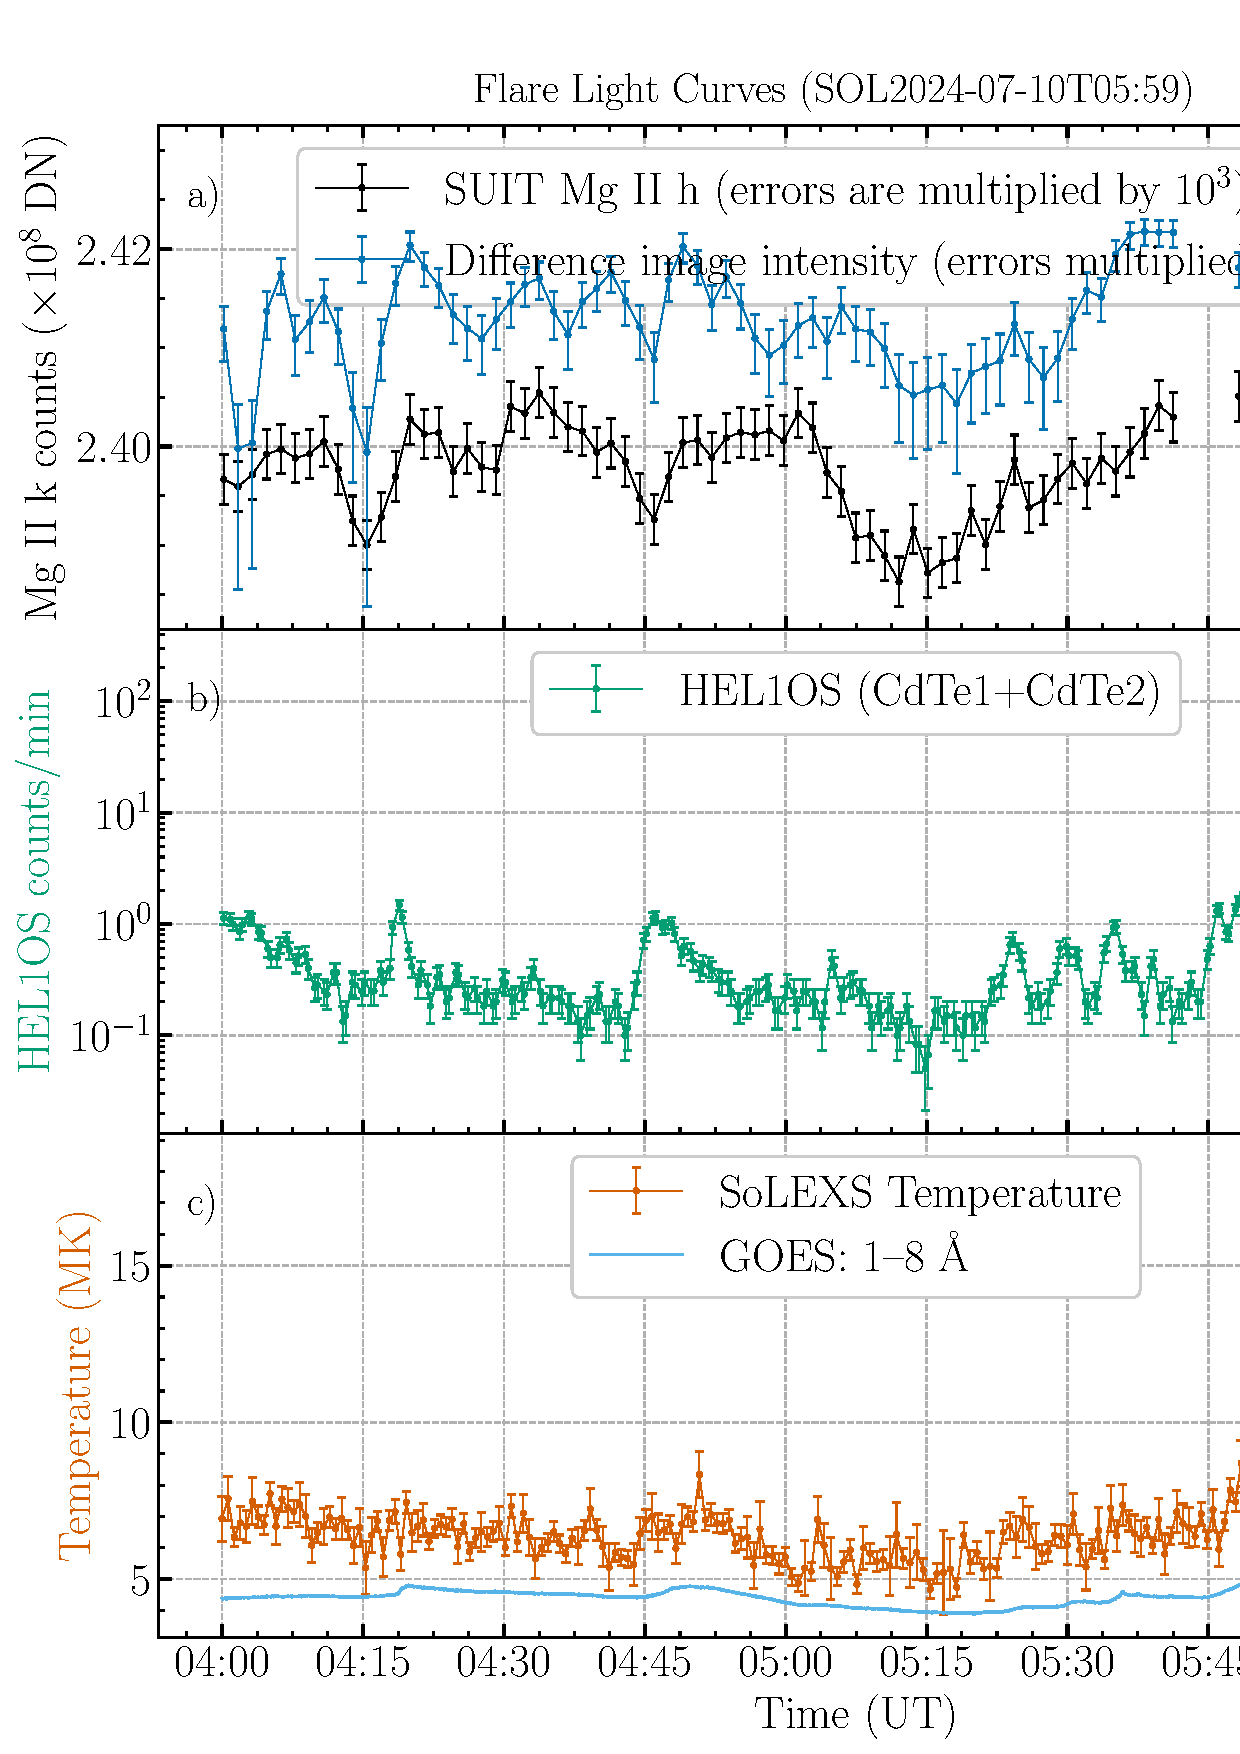
\includegraphics[width=1\linewidth]{Figures/case4_lc.pdf}  
    \caption{a) Total intensity light curve of the \ion{Mg}{ii} h ROI images (black). The errors of the individual data points are scaled by $10^3$ for visibility. The light curve of the difference-image intensity above the threshold is shown in cyan, with errors scaled by $10^4$ for clarity. b) HEL1OS light curve (CdTe 1 and CdTe 2, 9{--}40 keV), binned to 1-minute intervals, c) Temperature derived from SoLEXS(orange) and X-ray flux from the GOES 1{--} 8 {\AA} band (sky blue) }
    \label{fig:enter-label}
\end{figure}

\begin{figure}
    \centering
    \includegraphics[width=1\linewidth]{Figures/c4_plot_time_stamps.pdf}
    \caption{Case 4 : SUIT time stamp images of pre-flare enhancements }
    \label{fig:placeholder}
\end{figure}

\begin{figure}
    \centering
    \includegraphics[width=1\linewidth]{Figures/c4_hmi_plot_time_stamps.pdf}
    \caption{Case 4 HMI images, gray colour line represents PIL (0 Gauss value pixels)and green colour contours are SUIT enhancement contours from difference image.}
    \label{fig:c4_hmi}
\end{figure}


\subsection{Identifying pre-flare enhancements in SUIT}
To identify the pre-flare enhancements, we adopted the base-difference method. The base image was constructed using the median of the first five images in the 2-hour pre-flare image sequence, which also minimises first-frame selection bias.
The base-difference images contain quiet-Sun and plage-related fluctuations, as well as intensity fluctuations caused by the contamination pattern. To mitigate these effects, we had to set a threshold to see strong enhancements. 
Mean and standard deviation of the image were affected by bright events.
Therefore, we computed the median and standard deviation($\hat{\sigma}$) from median absolute deviation (MAD) of the difference image, which are less affected by bright events. And we applied the detection threshold given in Eq.~\ref{eqn:threshold} to the base-difference image, and contours were drawn around the regions exceeding this threshold.
\begin{align} \label{eqn:threshold}
\text{Threshold} &= \mathrm{median} + 5 \hat{\sigma}\\
\hat{\sigma} &= k \times \mathrm{MAD}
\end{align}

\noindent
where
\begin{align*}
%\text{For difference image intensity Xi}
\tilde{X}    &= \mathrm{median}(X_i)\\
\mathrm{MAD} &= \mathrm{median}\left(|X_i - \tilde{X}|\right)\\
\mathrm{k}	&\approx 1.4826 ~ \text{(for normal distribution)}
\end{align*}

Additionally, we imposed a size constraint of 16 pixels (corresponding to a PSF FWHM of$\approx$ 8 pixels). Only features larger than the PSF were retained. The base-difference total intensity within these selected regions was then used to generate the enhancement light curve.

\subsection{HEL1OS light curves}
To study simultaneous coronal activity, we consider the HEL1OS observations, which cover both thermal and non-thermal parts of the flare (10{--}40 keV).
Multiple count enhancement is observed in the 2-hour pre-flare window, but since it is a sun as a star observation, we cannot say the source is the same active region being observed from SUIT.
In most cases, we observe that SUIT enhancement is with by HEL1OS enhancements.
These enhancements could be small flares; if these enhancements are flares, we expect some non-thermal emission from them. But we have very few counts; we had to integrate over a few minutes to have enough counts to fit the spectra. 
However, as we integrate over a large time range, we obtain an averaged spectrum, which is essentially a first-order approximation. 
We compare our estimation with STIX for cases 5 to 10. which is described in section 4.

\subsection{Temperature from SoLEXS}
For the same pre-flare interval, we derived the emission measure and temperature from SoLEXS observations, assuming an isothermal plasma. 
We had to bin the data for about 2-3 minutes to have enough signal for calculation.
SoLEXS temperature follows almost the trend of HEL1OS.

\subsection{Identifying X-ray Source locations on full disc }
Both HEL1OS and SoLEXS observations come from the Sun as a star observation.
We are not sure of the source location of these small enhancements. Using the AIA observation, try to locate the source of these emissions (at least to the active region). 
AIA 131 \AA and AIA 94 \AA observe the hot plasma close to the X-ray in the SDO channels.

\begin{figure}
    \centering
    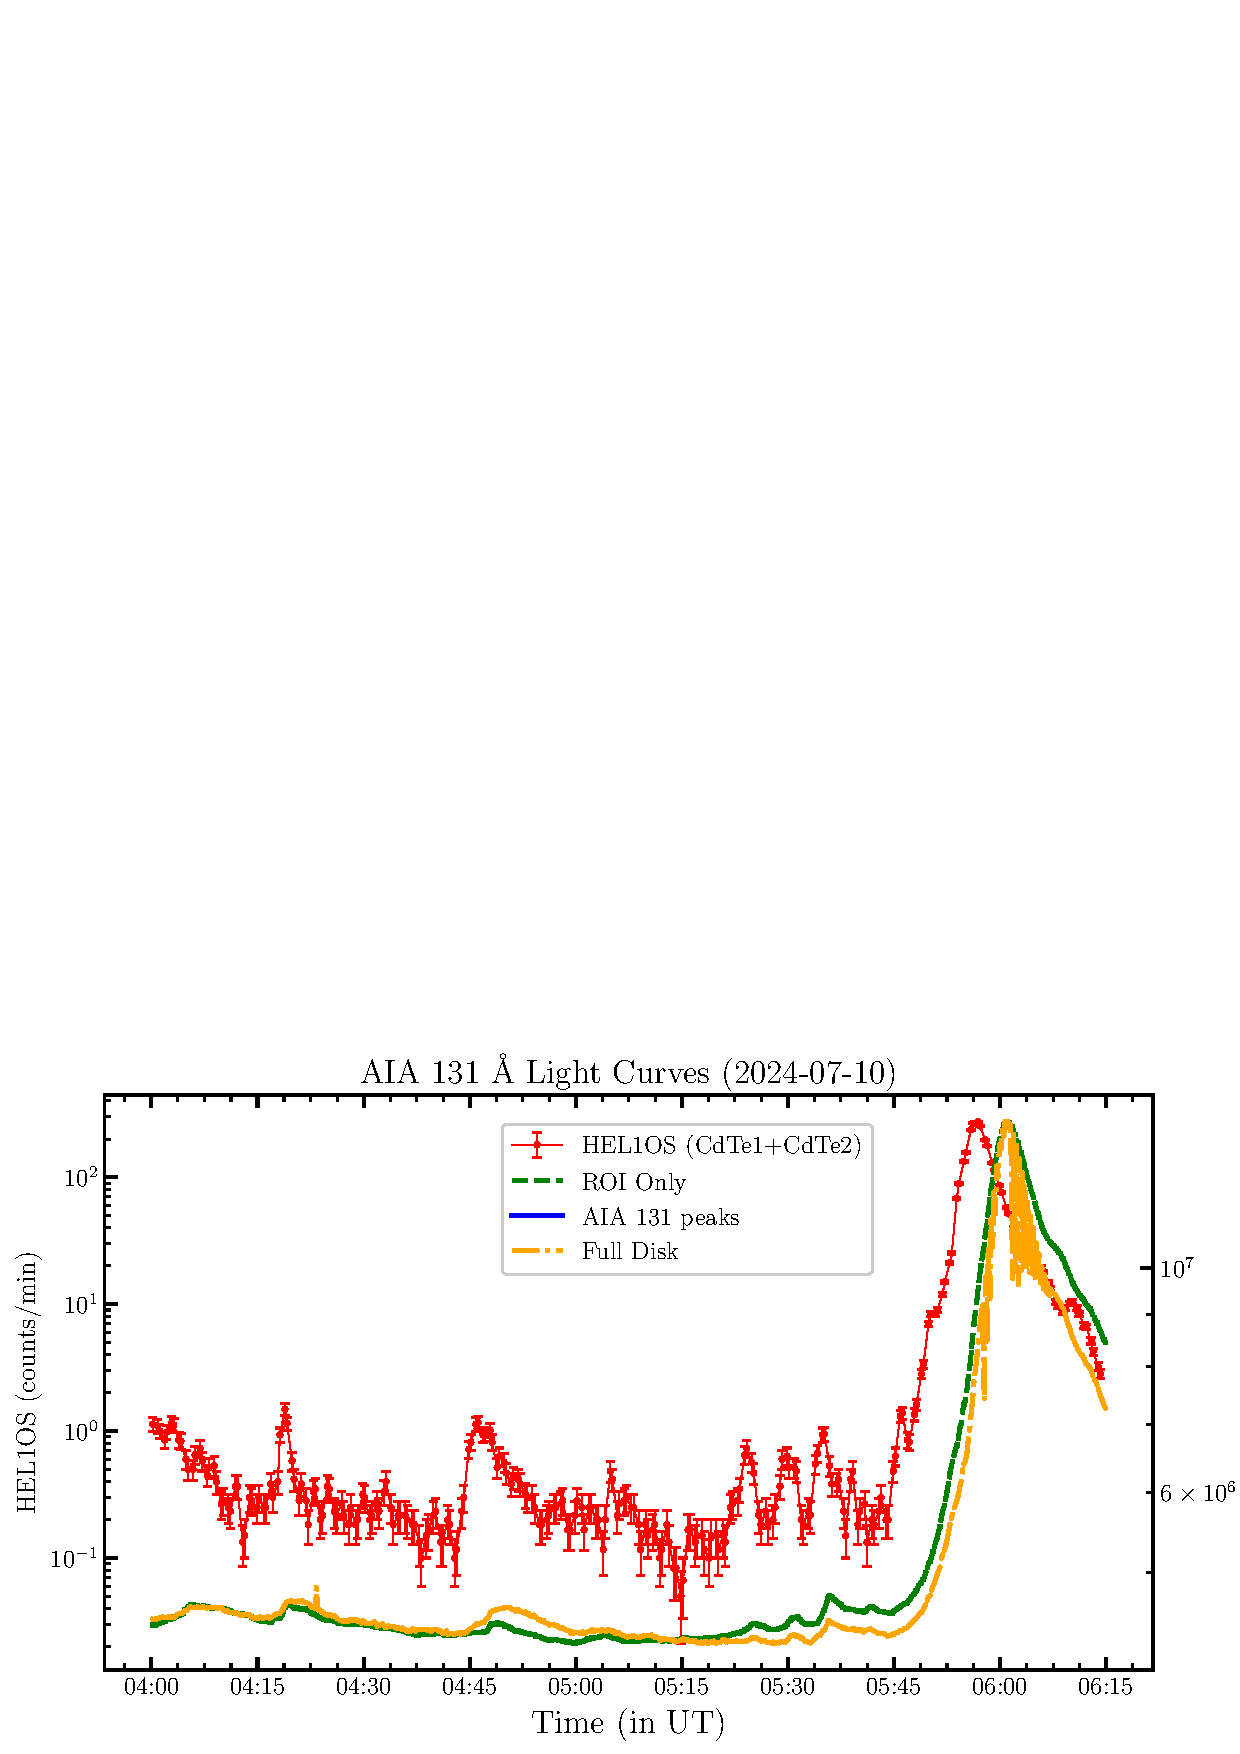
\includegraphics[width=1\linewidth]{Figures/c4_helios_aia_131_fd_roi_lc.pdf}
    \caption{AIA 131 light curves compared with HEL1OS light curve}
    \label{fig:placeholder}
\end{figure}

We plotted the total counts from the full Sun up to 1.1 \(R_\odot\), the active region of interest (ROI) observed with SUIT, and the HEL1OS counts. The full-disc light curve is expected to mimic observations of the Sun as a star in X-rays. 
We observe a slight delay between HEL1OS and AIA 131 light curves, most likely due to a difference in the energy bands of observation.
Each enhancement/event in HEL1OS can be connected to one active region (see the figure in the appendix, which includes all light curves).
This figure indicates which part of the X-ray light curve should be used to infer information about the active region being observed.


\subsection{Spectral analysis of pre-flare enhancements}
Currently, the HEL1OS counts are insufficient to fit the spectra, and with STIX spectra, we are analysing pre-flare enhancements.

\subsection{Hot onset cases}
In most of the flare cases, we observe elevated temperatures during flare onset in SoLEXS.  We also notice HEL1OS counts increasing during that period. 
This appears like a hot onset (previously reported, \cite{hudson_hot_2021},\cite{hudson_anticipating_2025}, \cite{battaglia_existence_2023})
We don't have enough counts in HEL1OS to conclude that they are of pure thermal nature. 
but, we have an STIX observation for the last 6 cases; using STIX data, we analyse the pre-flare enhancements and hot onset part by fitting the thermal and non-thermal parts.

\section{Results}

\subsection{Case 4: M1.5 class flare on July 10 2024}
We observe multiple brightenings in the pre-flare time window (Fig. \ref{c4_lc}).All brightenings occur cospatially with the polarity inversion line (PIL) (A1, A2 ,A3..) , with some located within approximately 10 arcseconds of it. (fig \ref{fig:c4_hmi}). 
All enhancements are cospatial with AIA 171 images, suggesting thier connection with coronal events. Exact timing analysis with other images could not be done due to low cadence in SUIT.

Several of the enhancements exhibit corresponding pre-event signatures in HEL1OS, HEL1OS counts are not enough to do the spectral analysis. 
To confirm their source locations, we examined the AIA 131 Å images.
The continuous enhancement began to appear at the flaring location after 05:28, which is approximately 31 minutes before the flare's soft X-ray peak time (based on the GOES data).We can observe multiple small events in the same active region(confirmed by AIA 131 plot) in this period. 
The coronal temperature measured from SoLEXS reaches approximately 6 MK and shows a rapid increase after 05:46, which is about 15 minutes before the soft X-ray peak.

\subsection{Case 5: M1.1 class flare on July 10 2024} 
In this case as well, multiple brightenings are observed during the pre-flare phase. Four major brightening sites were identified, including the flare locations (B1, B2, B3, and B4). 
All brightenings are on or close to the PIL (Cannot differentiate the exact location due to the PSF size).

After 14:45 onwards continuous brightening is observed, B2 and B3 are constant contributors and B1 is pulsating, note that all three regions are connected (see 171 images in fig ).
SoLEXS temperature does not show much variation, it lies between 6-7 MK.

(add iris images)

\subsection{Case 6: X1.8 class flare on October 9 2024}
It is the strong flares in our dataset and it was a sigmoid flare (sigmoid flare ref).
Minor pre-flare activity was detected in this active region. A small brightening was observed at point C1.

\subsection{Case 7: M1.3 class flare on November 1 2024}
Similar to the other cases, we also observe pre-flare brightenings in this case. 
All significant brightenings originate around the flaring location—specifically those for which HEL1OS shows enhancements above the error bars. These pre-flare brightenings occur on and close to the polarity inversion line (PIL), whereas the main flare takes place exactly above the PIL.

Using AIA source-localisation techniques, we found that the X-ray peaks correspond to the same region identified in the SUIT observations. 
STIX spectra for this event show three significant peaks, all exhibiting non-thermal emission, indicating that these correspond to small flare events.

In this case, we do not observe a single continuously enhanced region; instead, the emission is pulsating, consistent with a series of small flares.

\subsection{Case 8: M2.0 class flare on November 1 2024}
Only one enhancement was observed in the pre-flare phase, on the flare location.
Pre-flare enhancement and flare are happening slightly away from PIL.
STIX spectral fit suggest that pre-flare enhancement happening at 13:13 is also a small flare.
Continuos enhancement started at he flare location and the loop foot point about 30 min erlier than the flare peak.

\subsection{Case 9: M1.0 class flare on November 13 2024}
Only two brightening was observed in pre-flare phase where one among was on the flare location.
STIX spectra confirm that small enhancement is the flare.
Small continous enhancement was observed before flare on the flaring location and it stopped just before the flare.



\subsection{Case 10: M1.7 class flare on November 13 2024}
One small enhancement was observed but actual flare was happened another location but still this active region responded, suggesting larger connectivity between active region.



Our pre-flare study suggests that multiple small brightening events are observed in the chromosphere before the flare. This could be due to a small flare or pure thermal events.

Most of the brightening is happening on the PIL, where a flare is going to take place.

All these small events are counter parts of coronal activity .

We observe that some of these events are not started in the same region but are a response to a small event that happened in another region of the sun.
This suggests a larger network connecting all active regions. 

Summary table
\begin{table*}
    \centering
    \begin{tabular}[t]{lccccr}
    \hline
     Case no. & Pre-flare brightening location & Nature of PFB & Hot onset (Yes/No) &Onset temperature& GOES Flare peak time\\
     \hline
     Case 4& Flaring location& Continuous & Yes & 6-7& 5:59\\
     Case 5& Flaring location and closeby & Continuous & No & 6-7& 15:39\\
     Case 6& Flaring location and closeby & Before flare & No & 6-7&01:56\\
     Case 7& Flaring location & Pulasting & No & 7-8 & 02:16\\

    \hline
    \end{tabular}
\end{table*}
\section{Discussion}
Multiple brightenings on the PIL were observed. It can also be a small flare, since it is solar maximum, not to be confused with just an enhancement and thought of as a precursor. 

All these multiple small events could lead to destabilising the larger active region and causing a flare.


especially the event happening just before a flare may be the subject of interest that can tell or that can be the signature of a flare.

Further investigation based on HMI could lead to much more concrete evidence for the flare trigger understanding.



\section{Conclusion}

Aditya-L1 can clearly demonstrate the capability of observing pre-flare dynamics in both the chromosphere and the corona by combining both imaging and spectral observations.

Repeating the same procedures during Solar minima could give further confidence in our results.

We need high cadence imaging spectrographs to isolate the source location for better understading of the solar corona during flares.

\section*{Acknowledgements}

Acknowledge TMA Pai Scholarship, MCNS, Sunpy, SUIT team, CfA people

%%%%%%%%%%%%%%%%%%%%%%%%%%%%%%%%%%%%%%%%%%%%%%%%%%
\section*{Data Availability}
All data are publicly available on the ISSDC-pradan website.





%%%%%%%%%%%%%%%%%%%% REFERENCES %%%%%%%%%%%%%%%%%%

% The best way to enter references is to use BibTeX:

\bibliographystyle{mnras}
\bibliography{example} % if your bibtex file is called example.bib


% Alternatively, you could enter them by hand, like this:
% This method is tedious and prone to error if you have lots of references
%\begin{thebibliography}{99}
%\bibitem[\protect\citeauthoryear{Author}{2012}]{Author2012}
%Author A.~N., 2013, Journal of Improbable Astronomy, 1, 1
%\bibitem[\protect\citeauthoryear{Others}{2013}]{Others2013}
%Others S., 2012, Journal of Interesting Stuff, 17, 198
%\end{thebibliography}

%%%%%%%%%%%%%%%%%%%%%%%%%%%%%%%%%%%%%%%%%%%%%%%%%%

%%%%%%%%%%%%%%%%% APPENDICES %%%%%%%%%%%%%%%%%%%%%

\appendix

\section{Justification for few steps}
\subsection{Difference image threshold}

\section{Flare light curves}


\begin{figure}
    \centering
    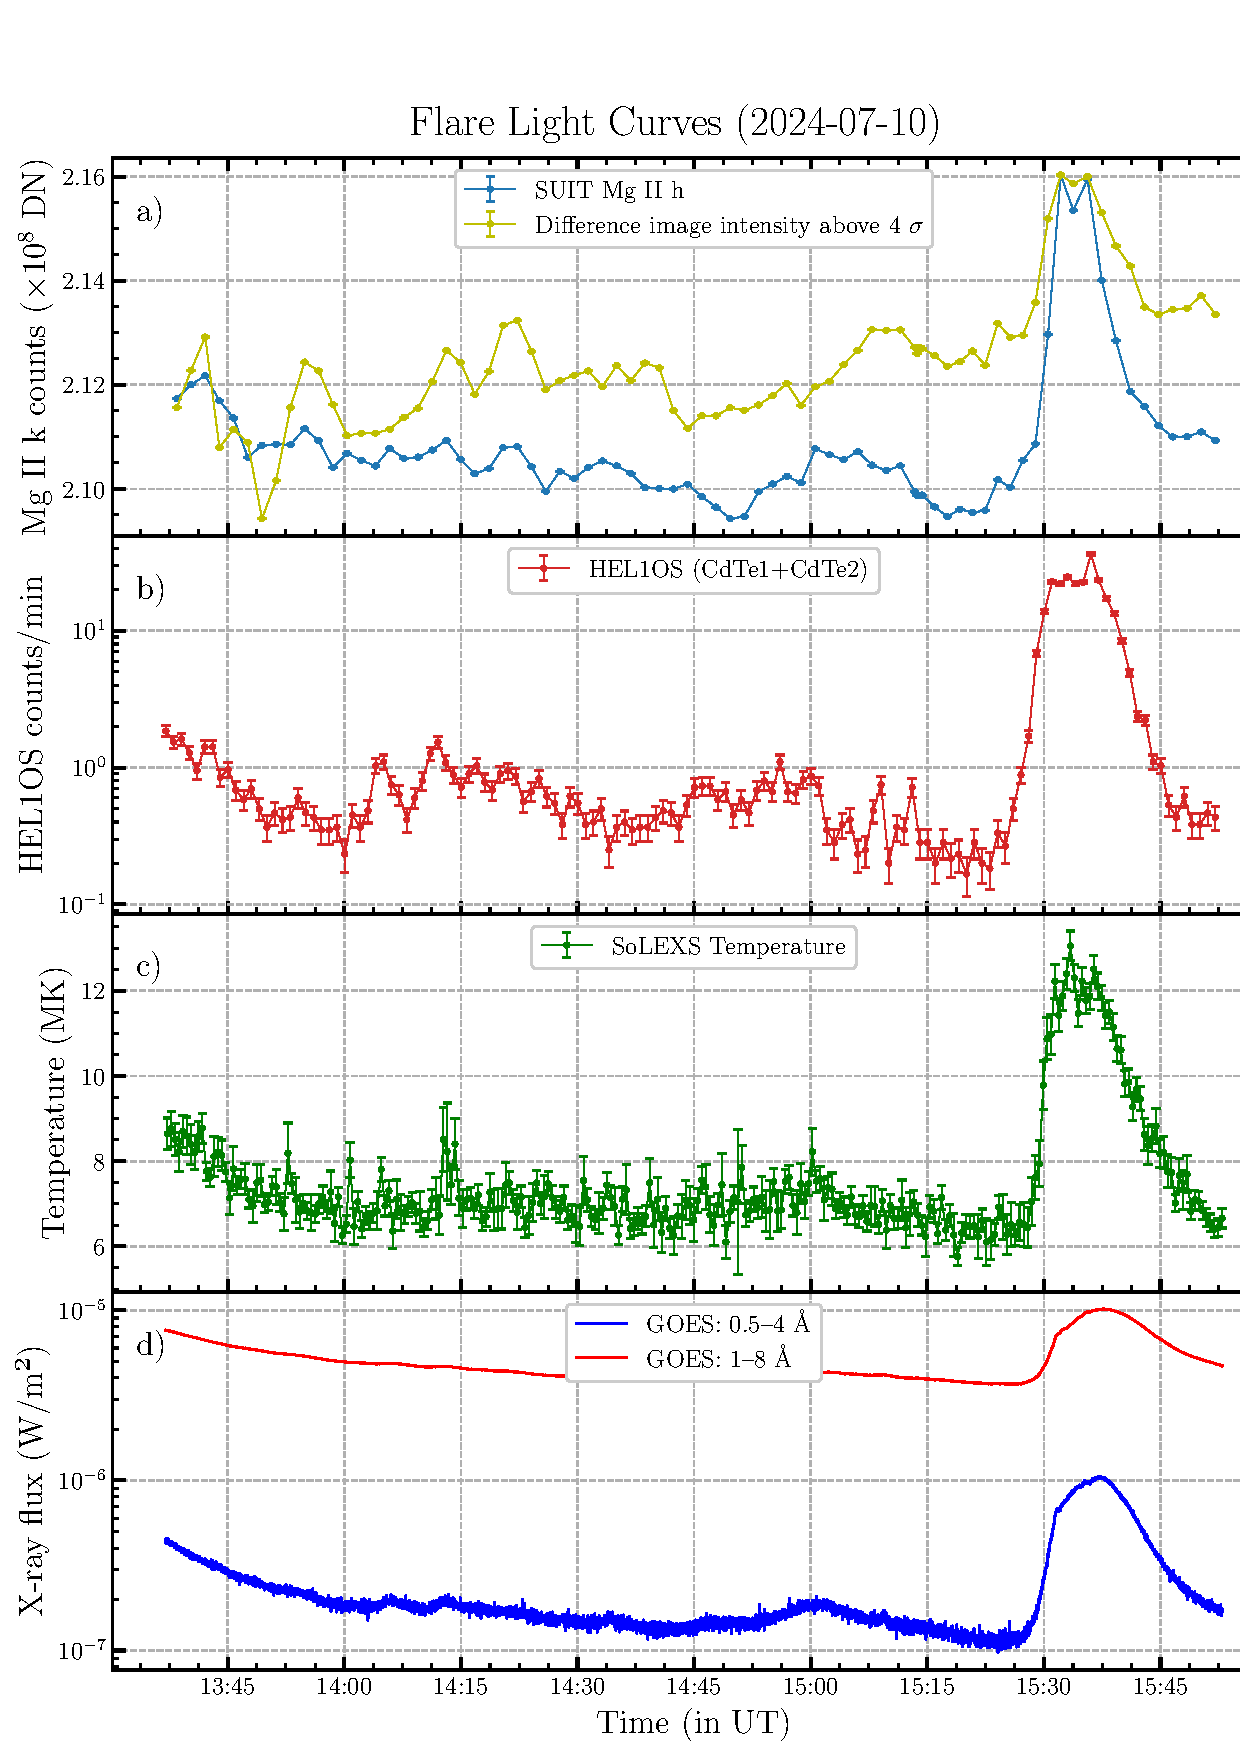
\includegraphics[width=1\linewidth]{Figures/case5_lc.pdf}
    \caption{Case 5 Light curves}
    \label{fig:placeholder}
\end{figure}

\begin{figure}
    \centering
    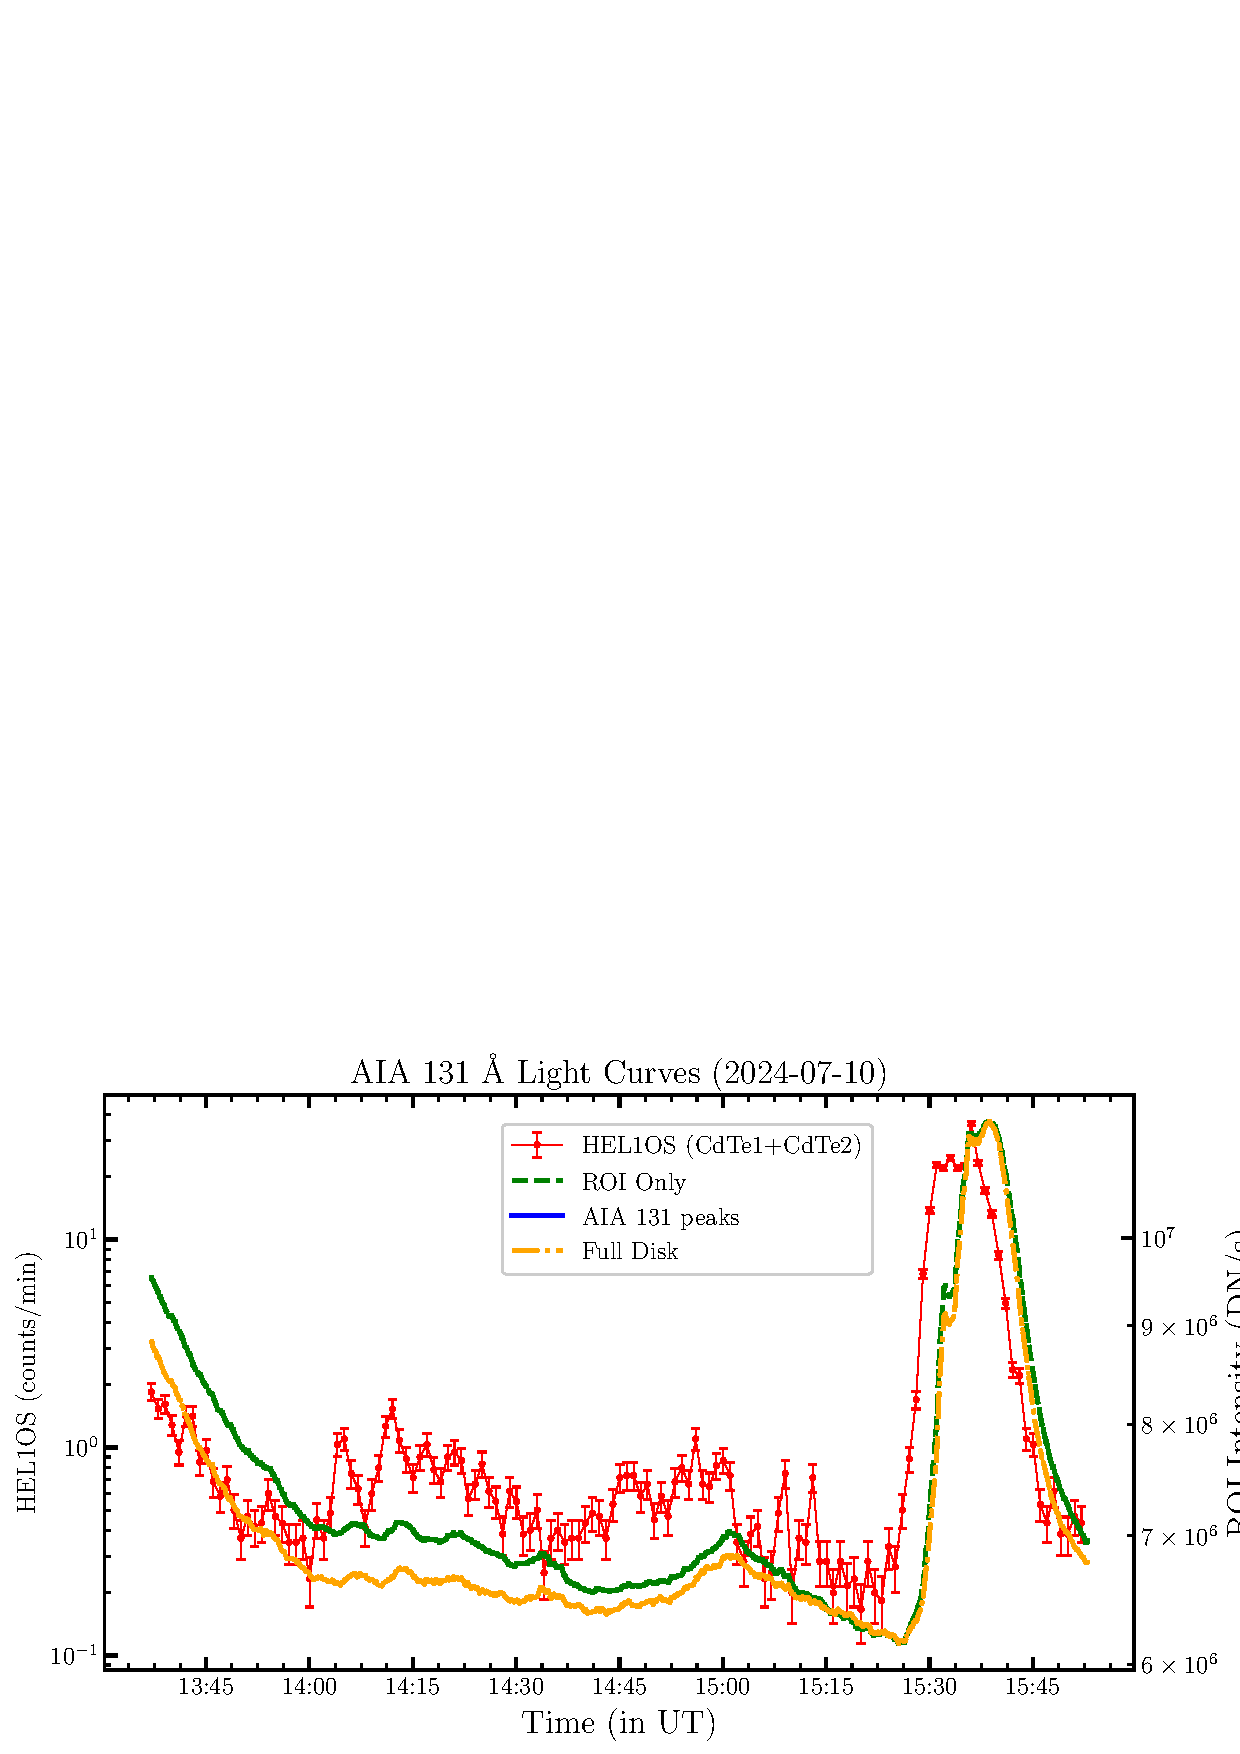
\includegraphics[width=1\linewidth]{Figures/c5_helios_aia_131_fd_roi_lc.pdf}
    \caption{Case 5: AIA 131 light curve}
    \label{fig:placeholder}
\end{figure}

\begin{figure}
    \centering
    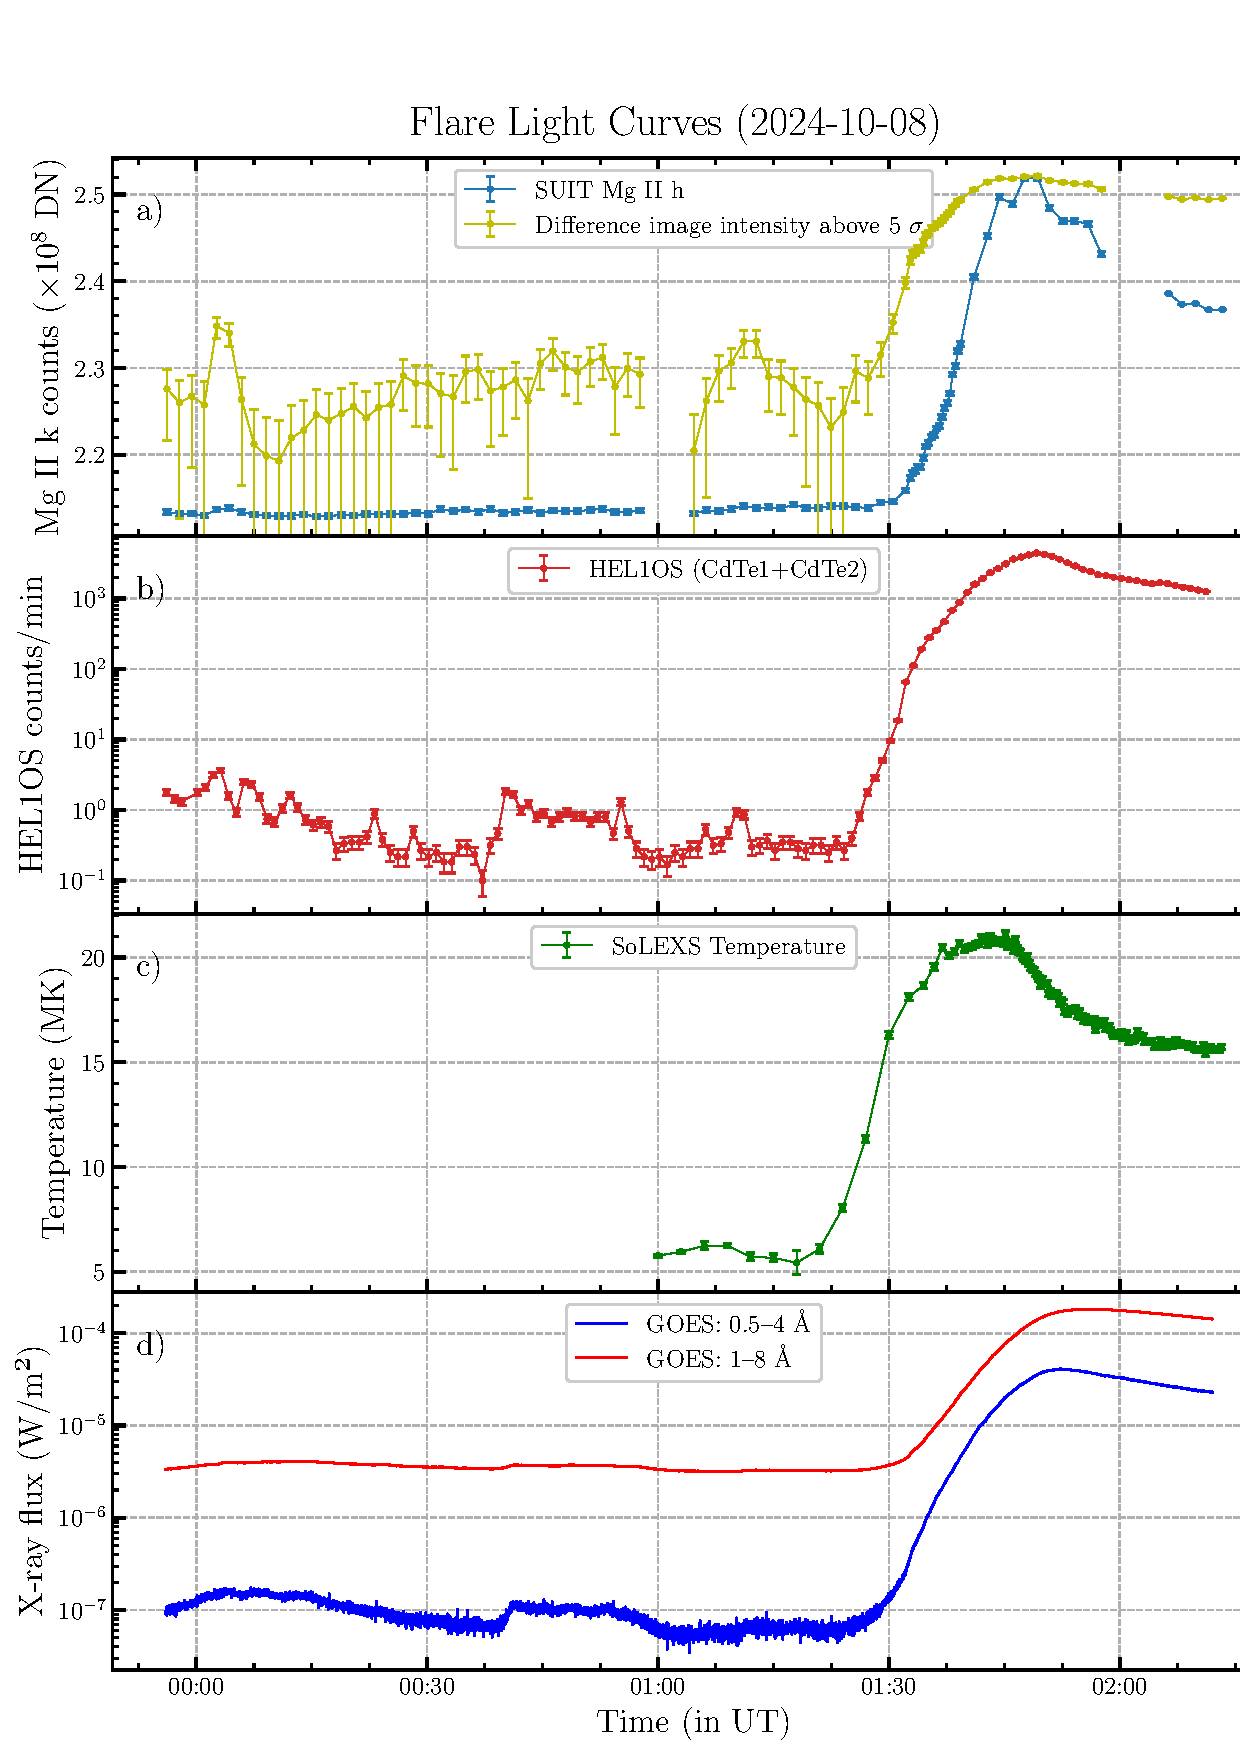
\includegraphics[width=1\linewidth]{Figures/case6_lc.pdf}
    \caption{Case 6 Light curves}
    \label{fig:placeholder}
\end{figure}

\begin{figure}
    \centering
    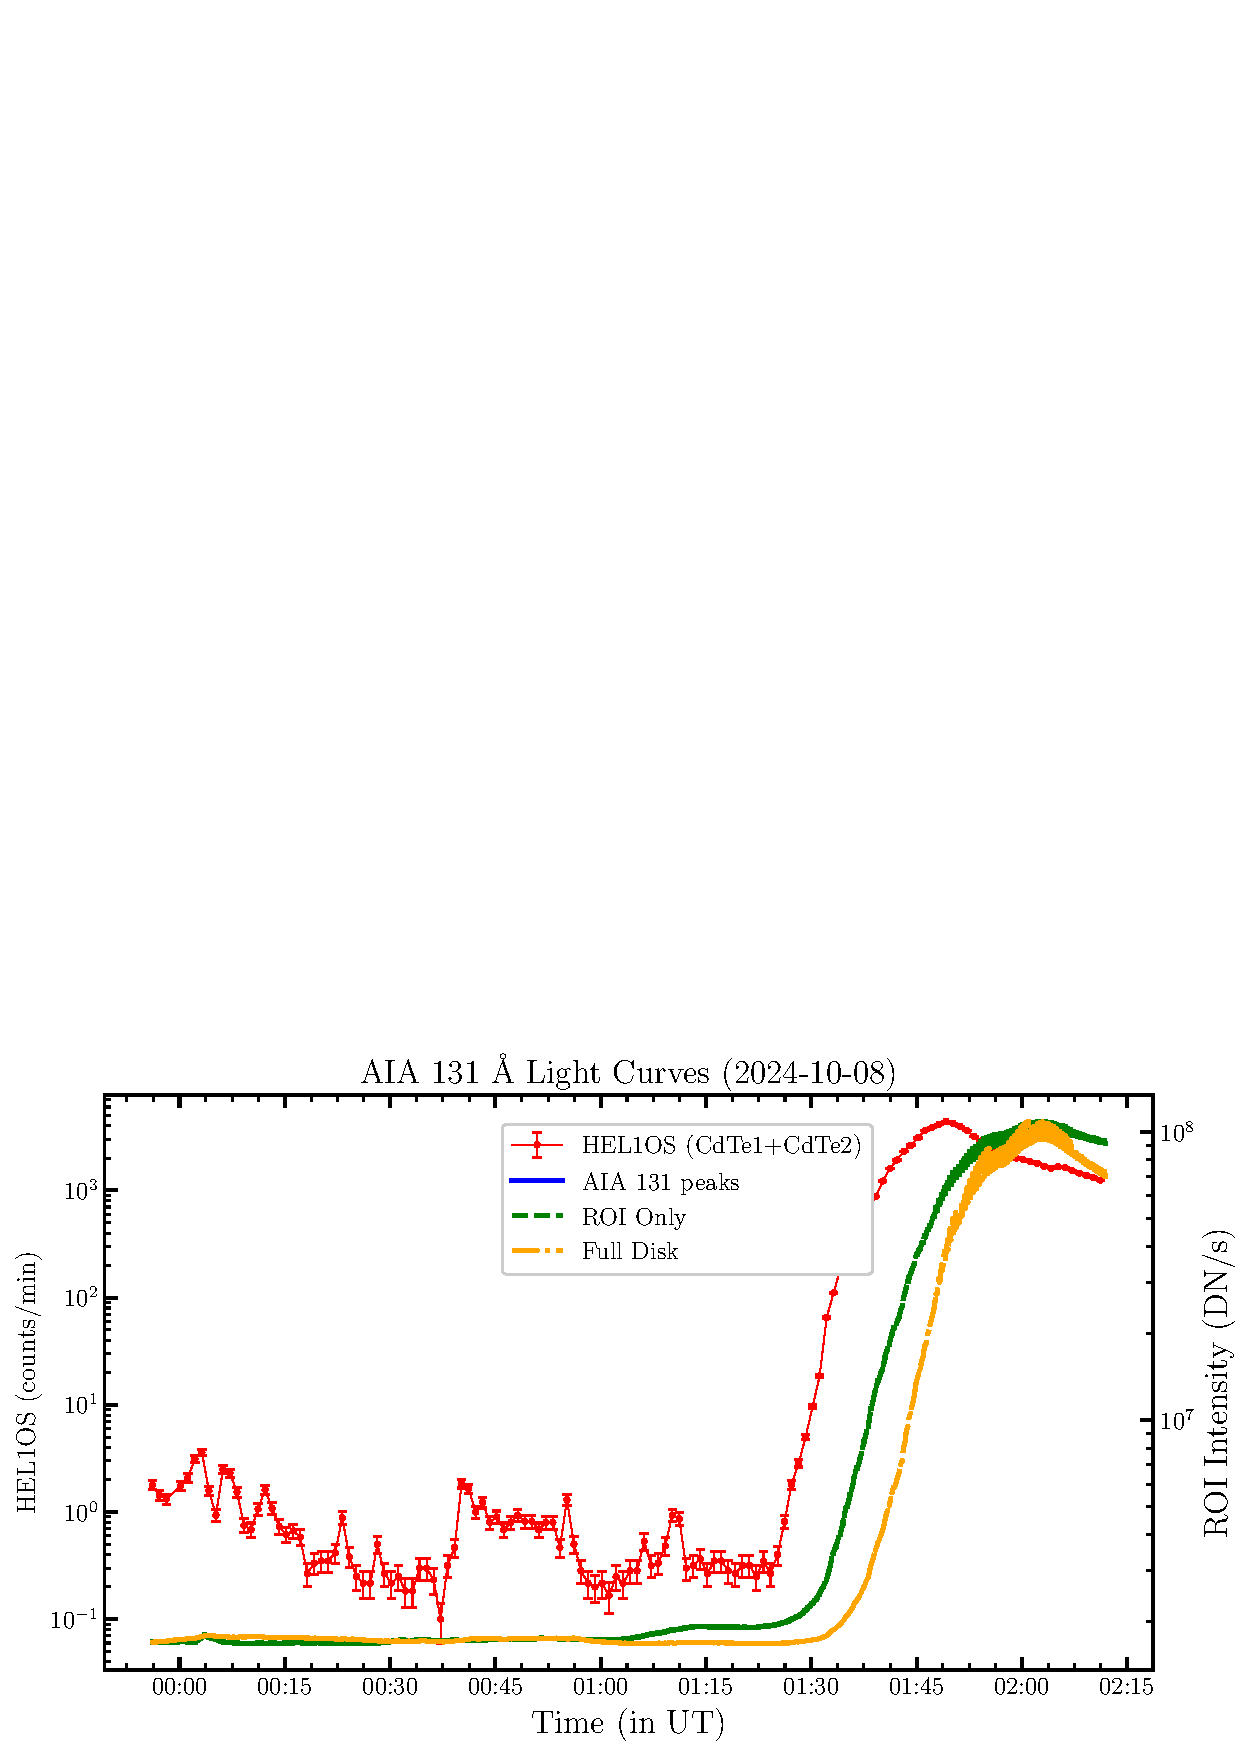
\includegraphics[width=1\linewidth]{Figures/c6_helios_aia_131_fd_roi_lc.pdf}
    \caption{Case 6: AIA 131 light curve}
    \label{fig:placeholder}
\end{figure}

\begin{figure}
    \centering
    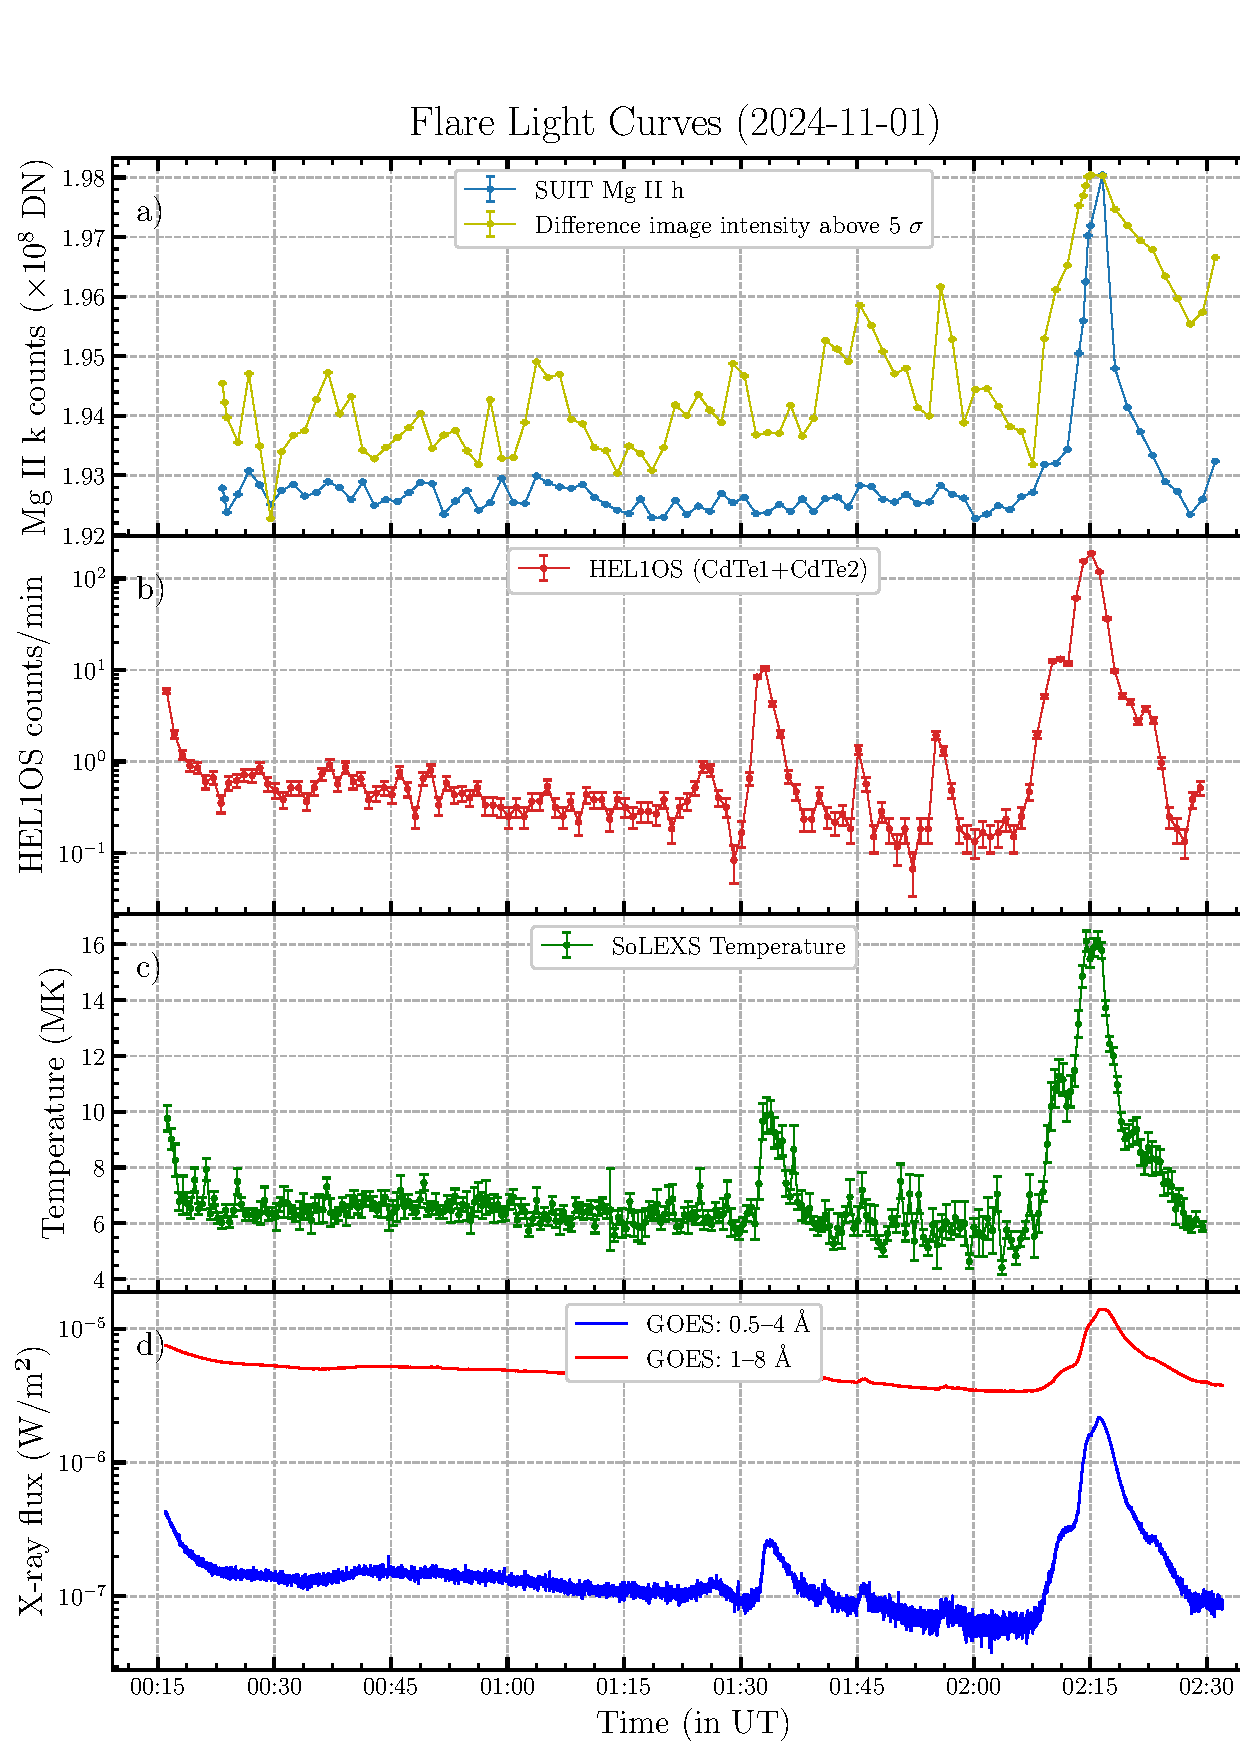
\includegraphics[width=1\linewidth]{Figures/case7_lc.pdf}
    \caption{Case 7 Light curves}
    \label{fig:placeholder}
\end{figure}

\begin{figure}
    \centering
    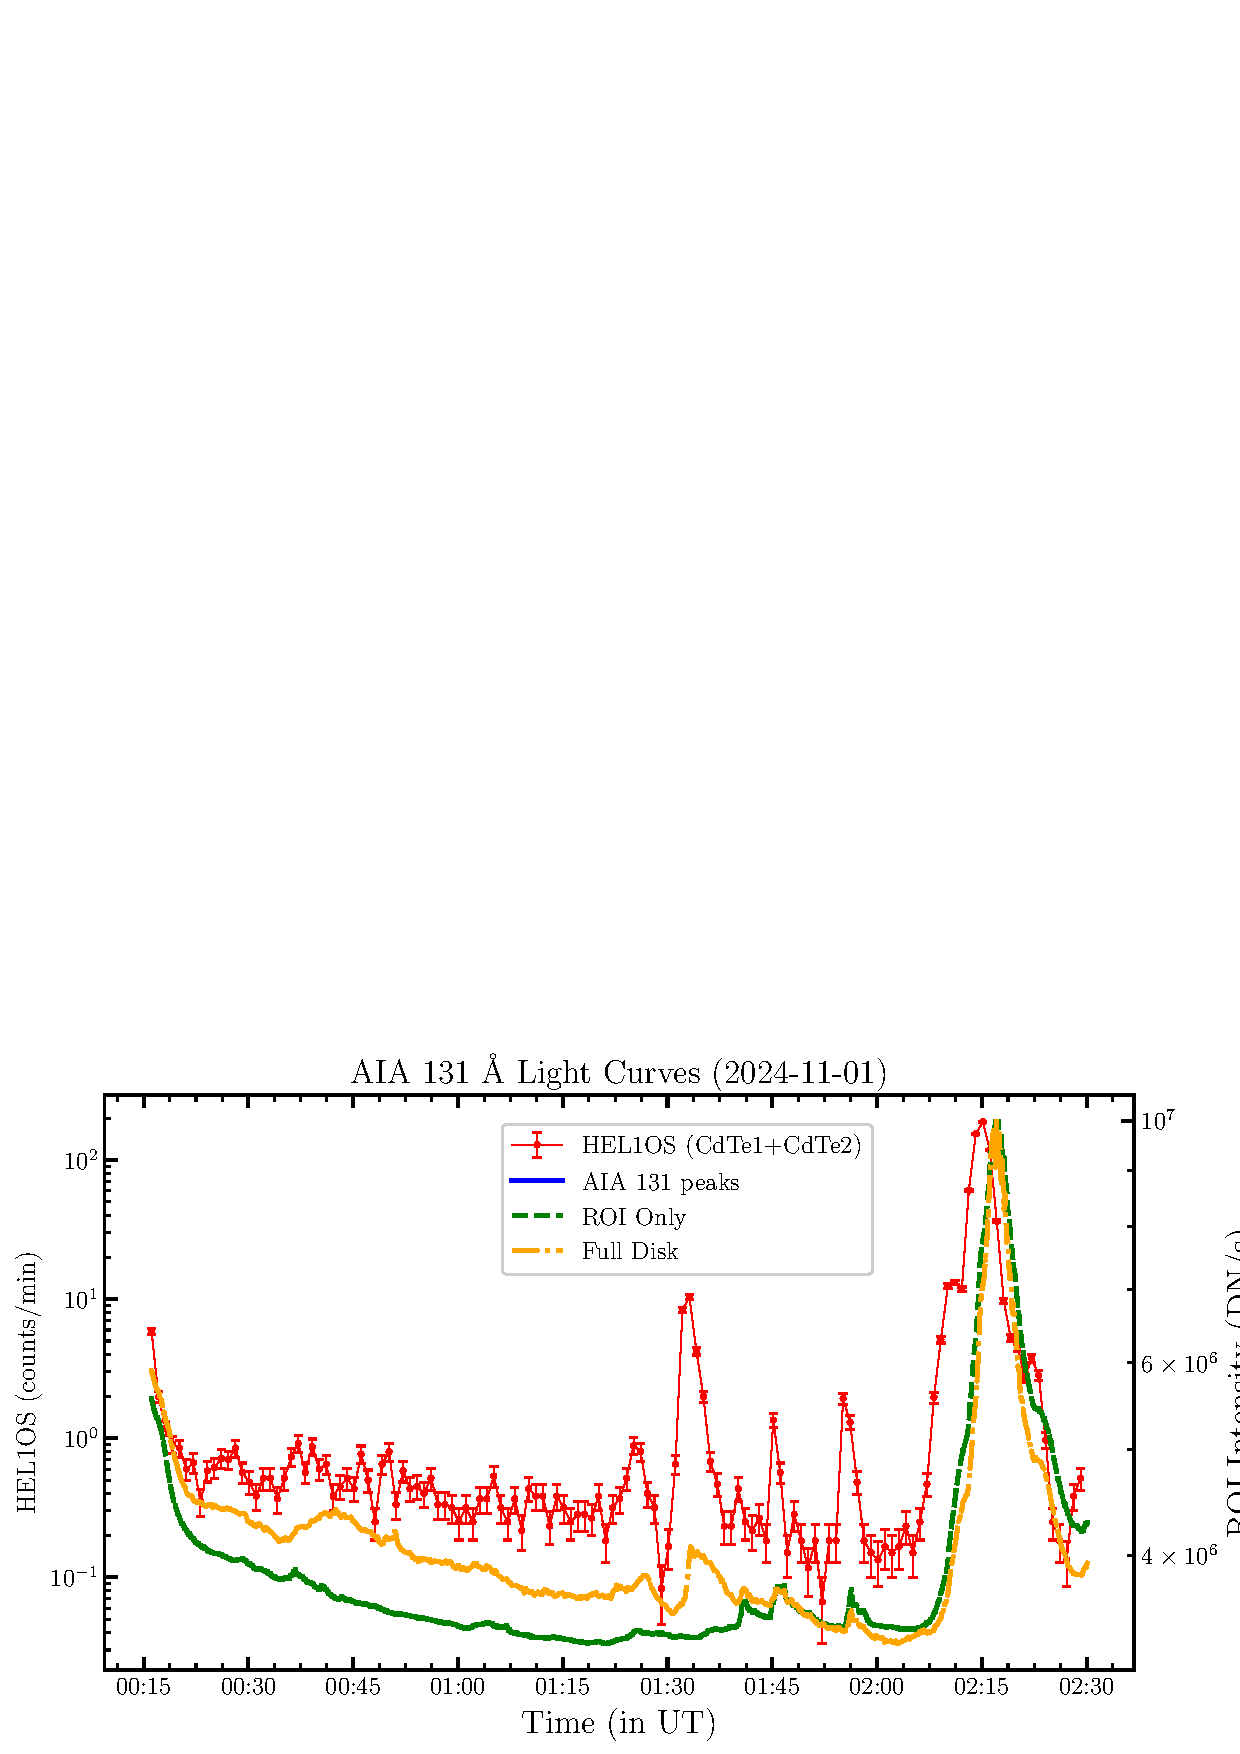
\includegraphics[width=1\linewidth]{Figures/c7_helios_aia_131_fd_roi_lc.pdf}
    \caption{Case 7: AIA 131 light curve}
    \label{fig:placeholder}
\end{figure}

\begin{figure}
    \centering
    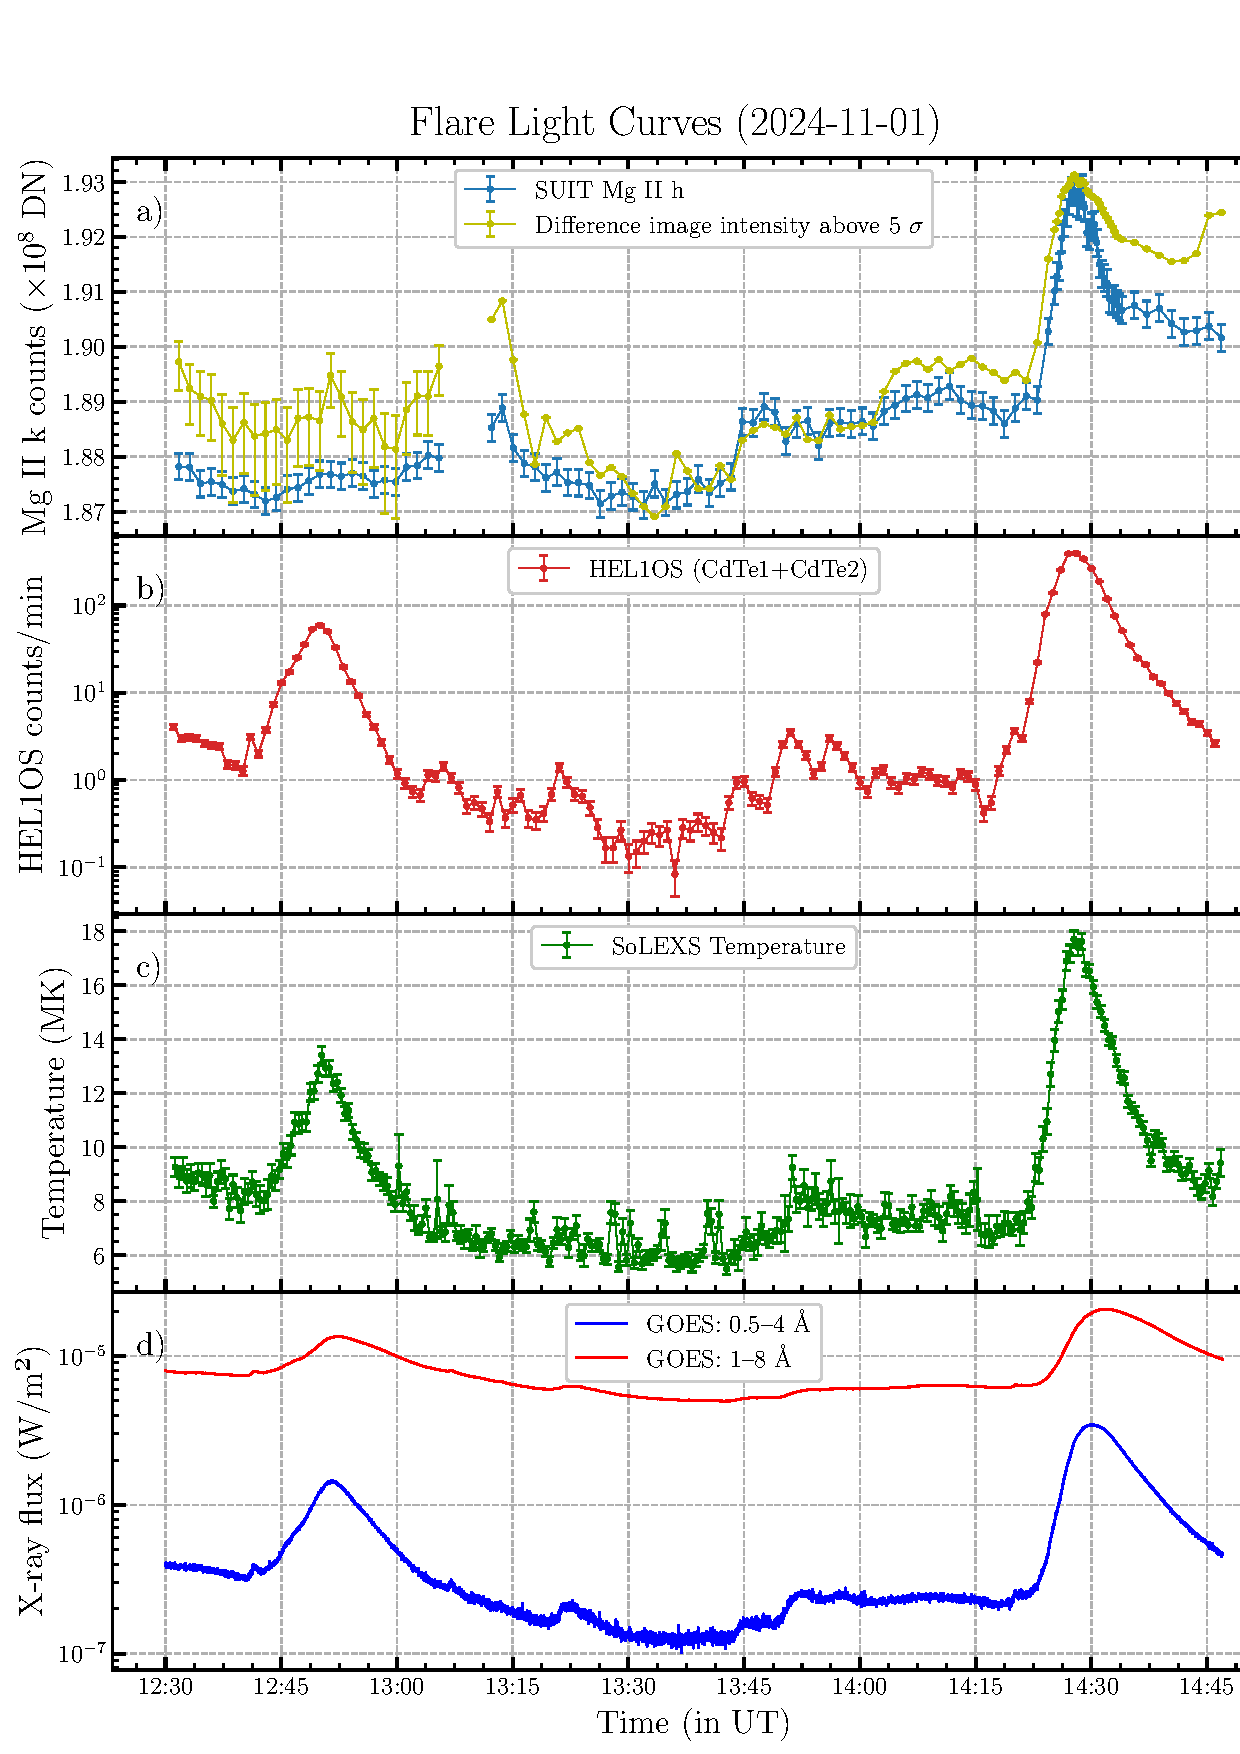
\includegraphics[width=1\linewidth]{Figures/case8_lc.pdf}
    \caption{Case 8 Light curves}
    \label{fig:placeholder}
\end{figure}

\begin{figure}
    \centering
    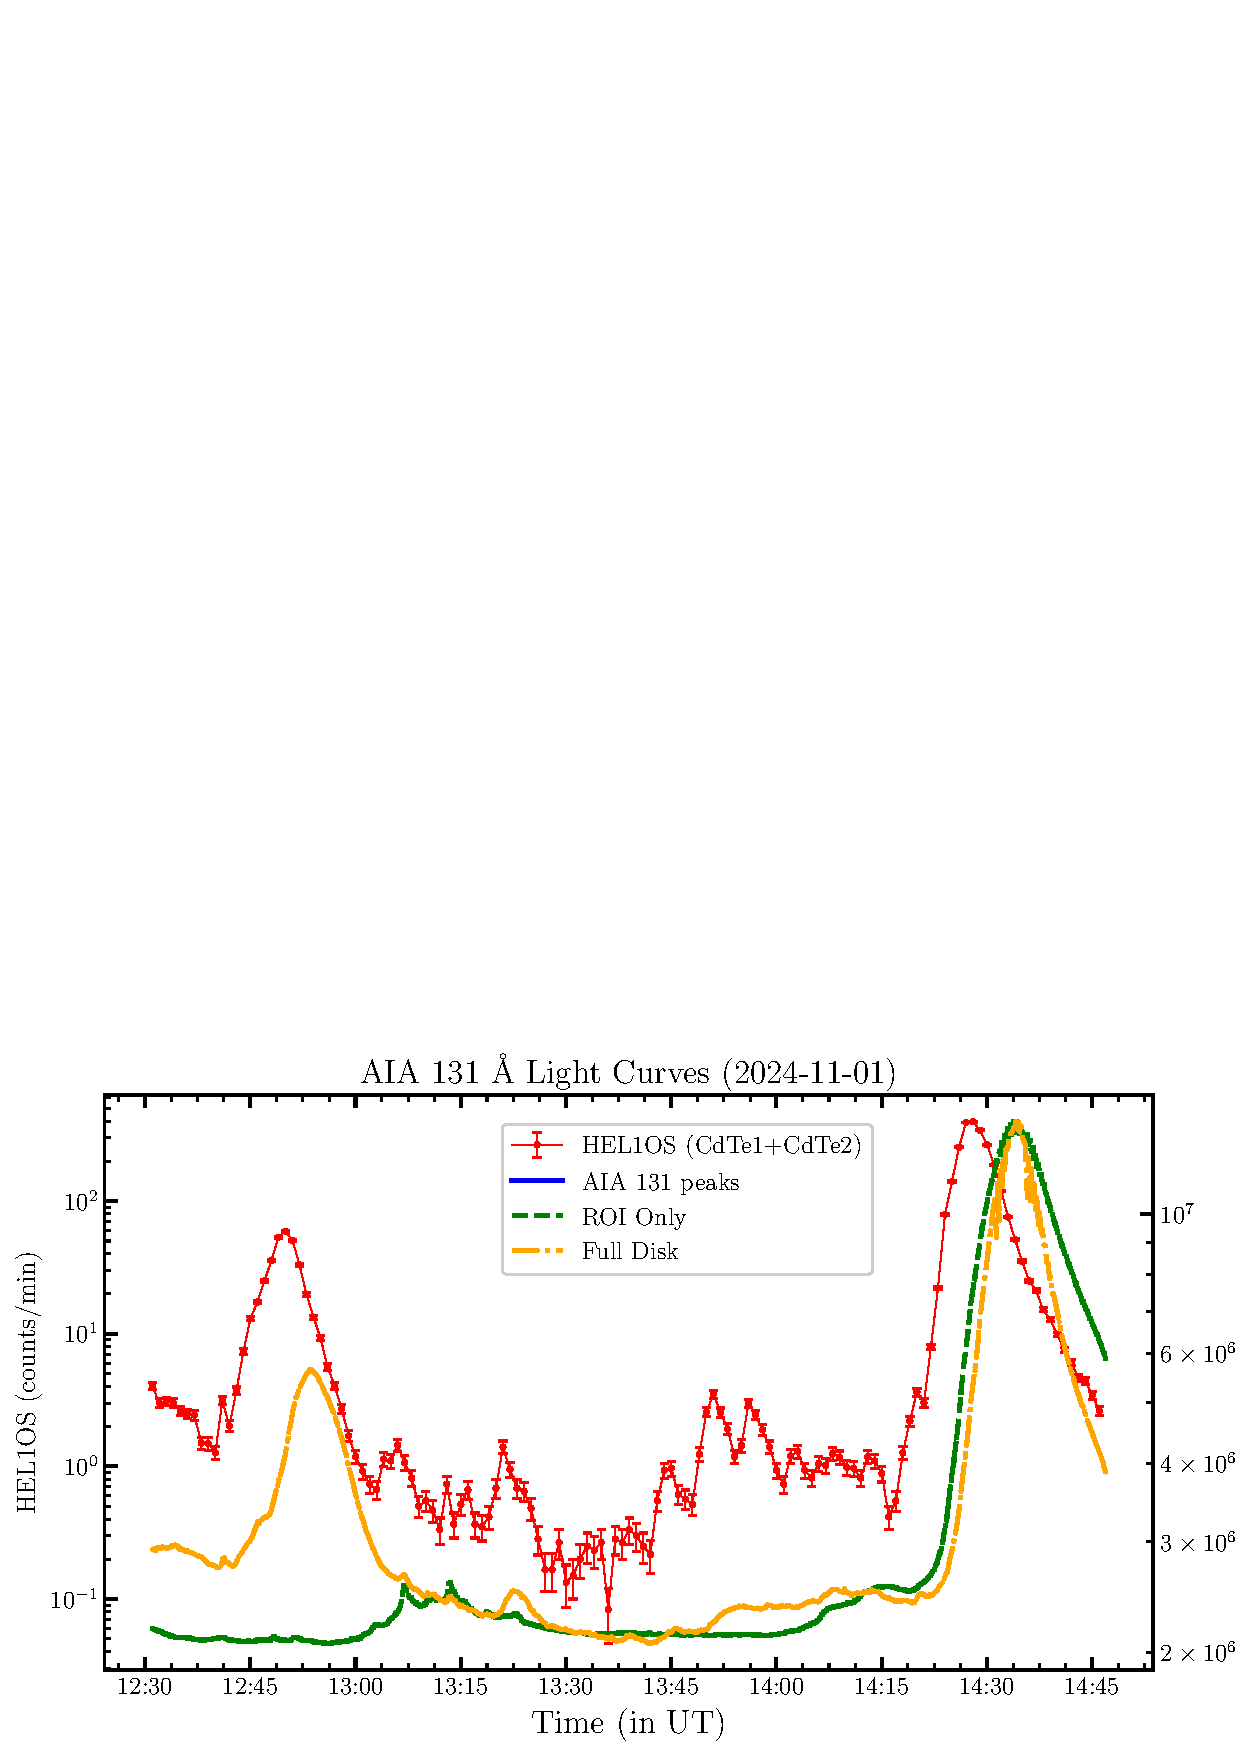
\includegraphics[width=1\linewidth]{Figures/c8_helios_aia_131_fd_roi_lc.pdf}
    \caption{Case 8: AIA 131 light curve}
    \label{fig:placeholder}
\end{figure}

\begin{figure}
    \centering
    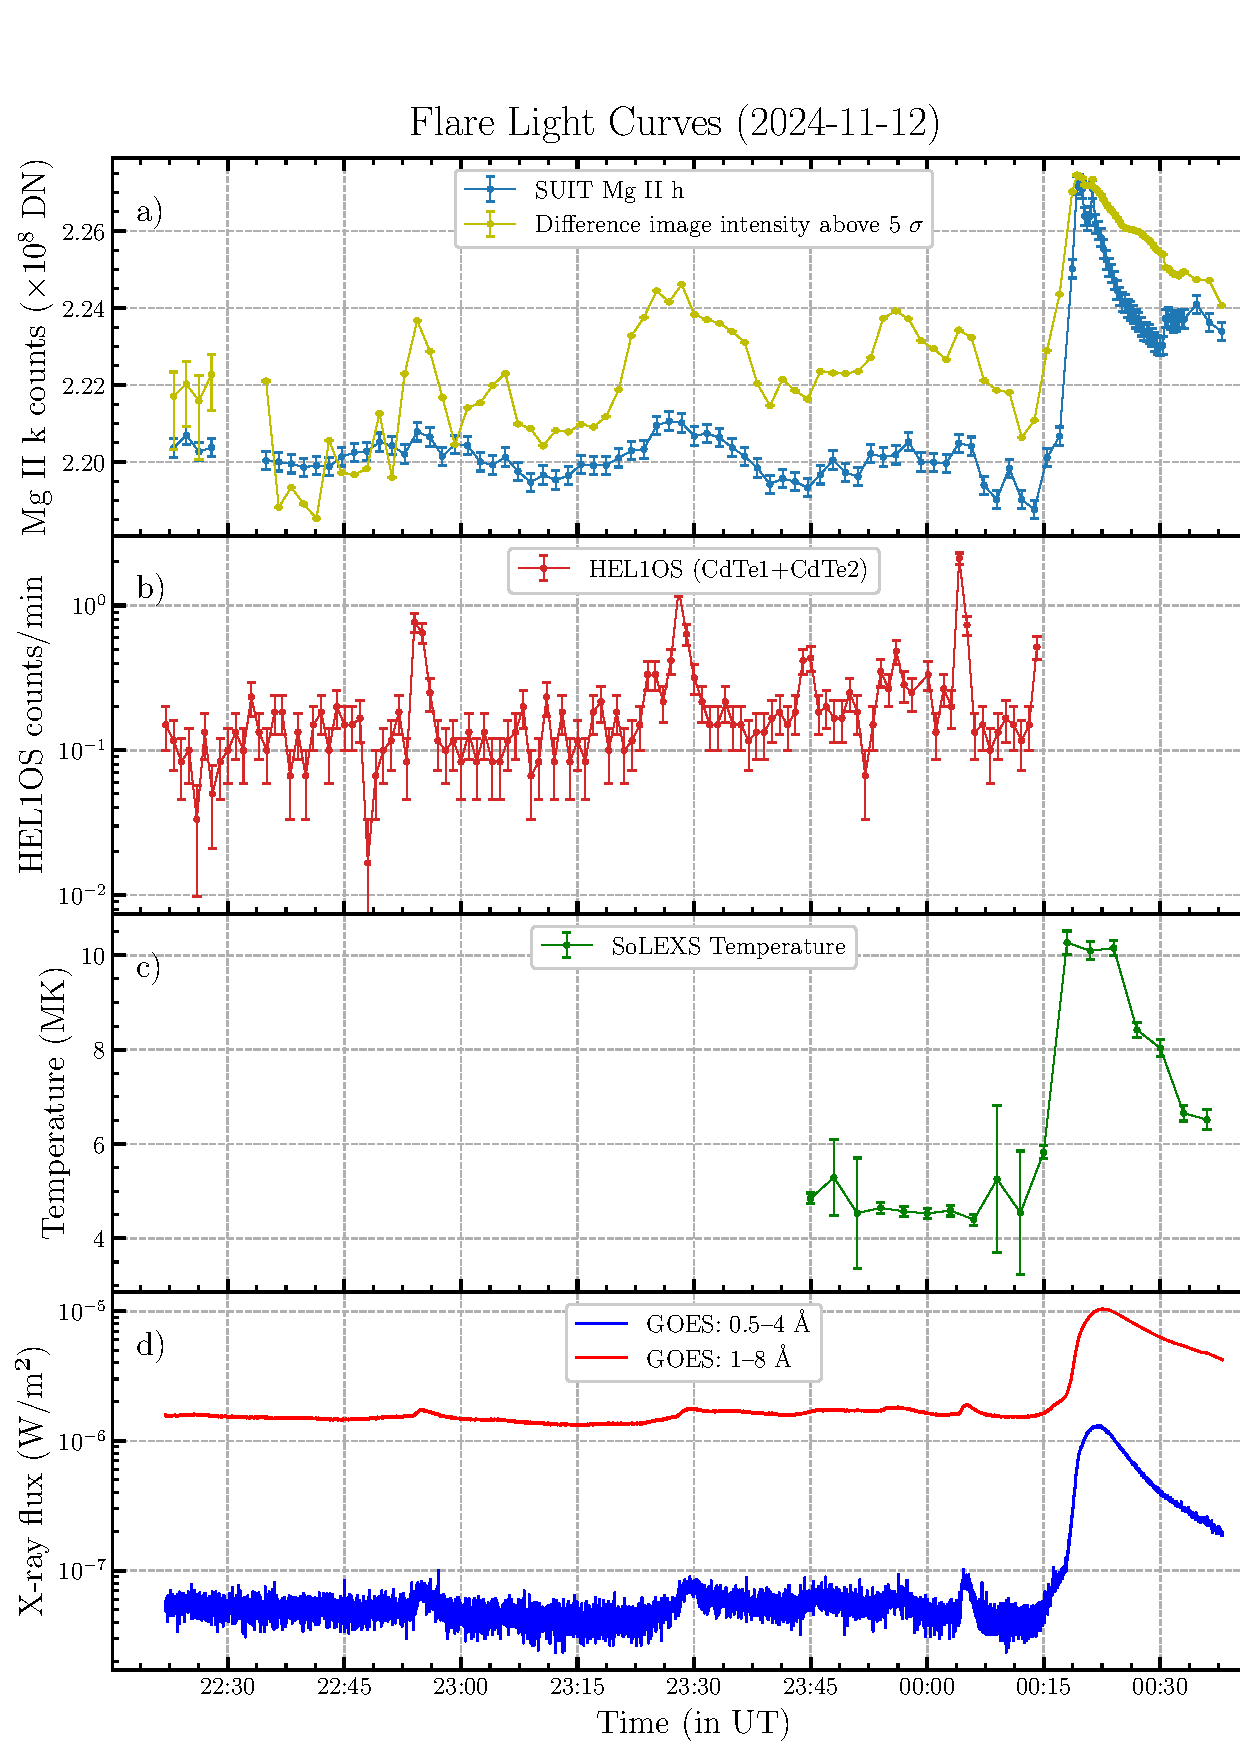
\includegraphics[width=1\linewidth]{Figures/case9_lc.pdf}
    \caption{Case 9 Light curves}
    \label{fig:placeholder}
\end{figure}

\begin{figure}
    \centering
    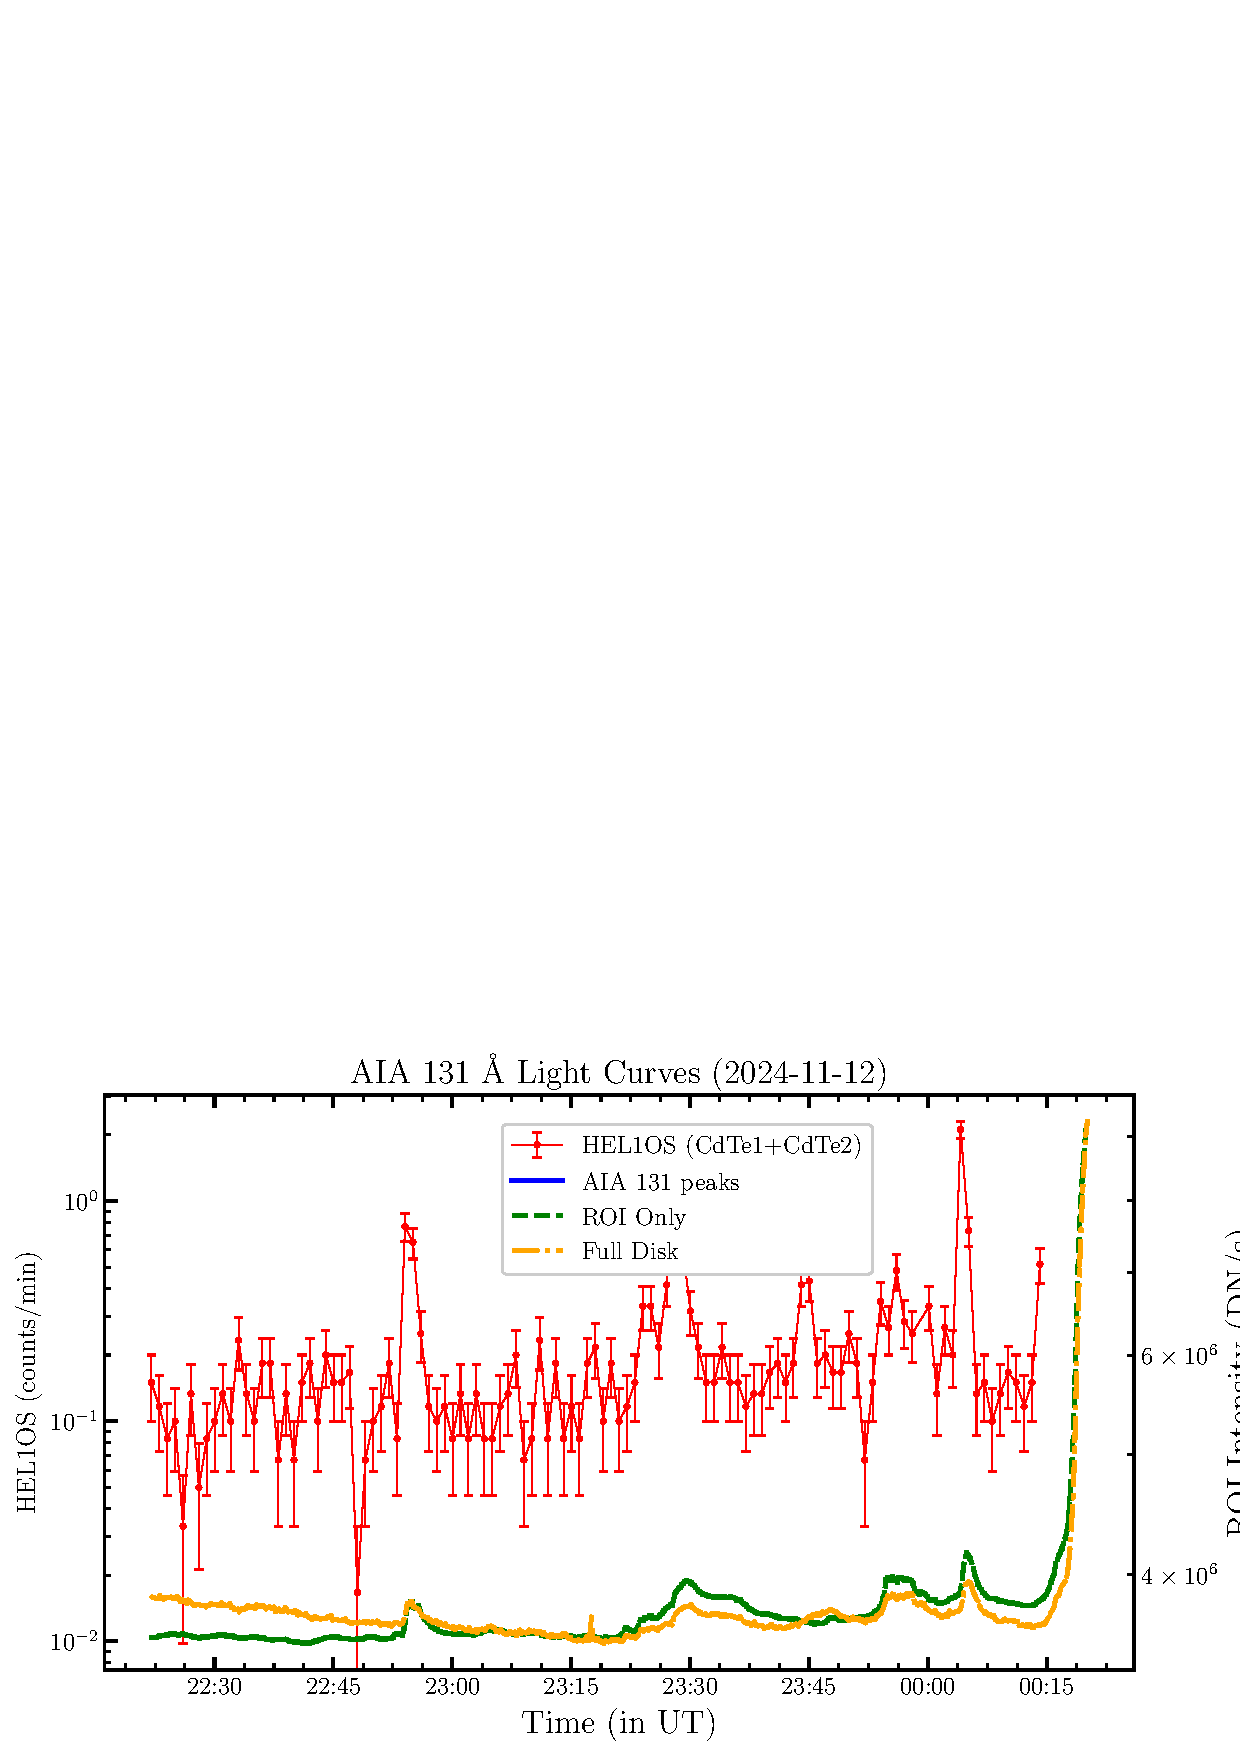
\includegraphics[width=1\linewidth]{Figures/c9_helios_aia_131_fd_roi_lc.pdf}
    \caption{Case 9: AIA 131 light curve}
    \label{fig:placeholder}
\end{figure}

\begin{figure}
    \centering
    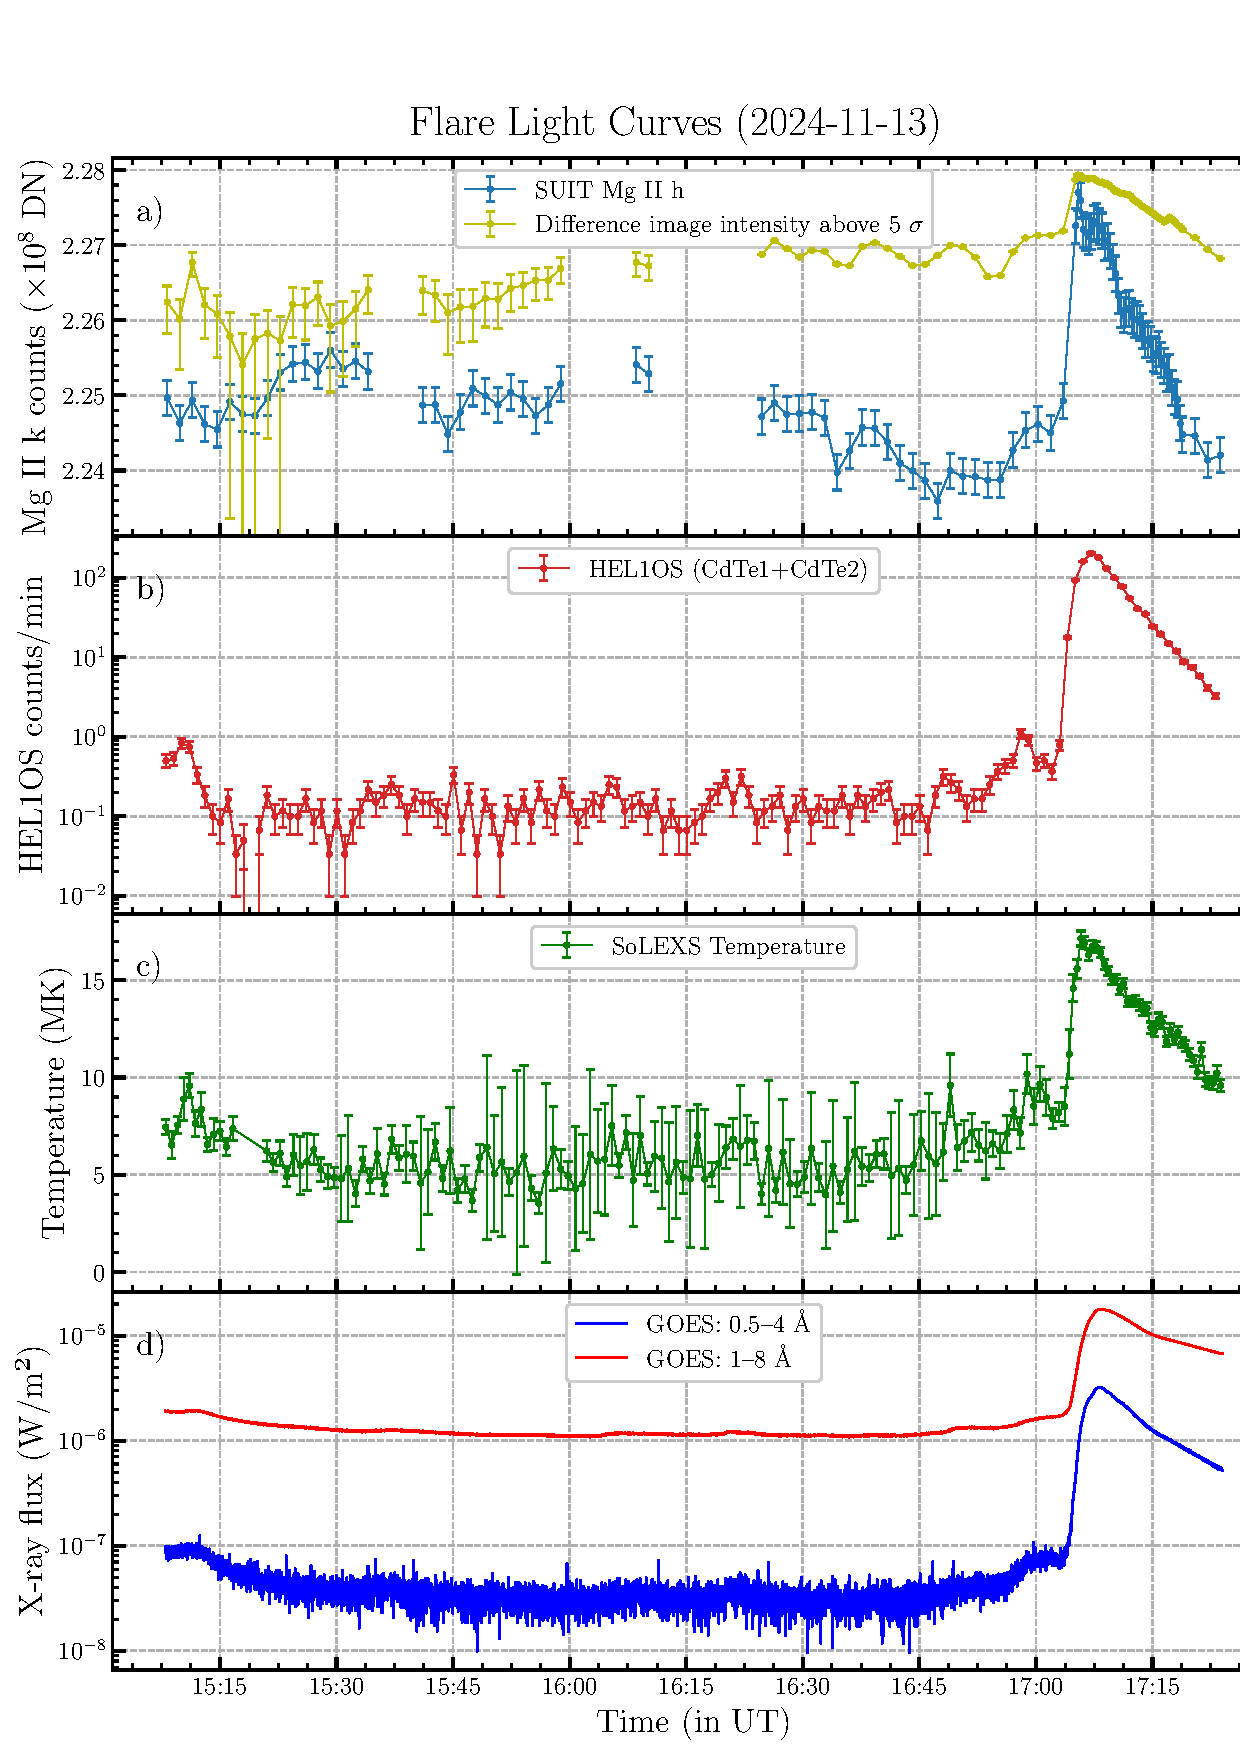
\includegraphics[width=1\linewidth]{Figures/case10_lc.pdf}
    \caption{Case 10 Light curves}
    \label{fig:placeholder}
\end{figure}

\begin{figure}
    \centering
    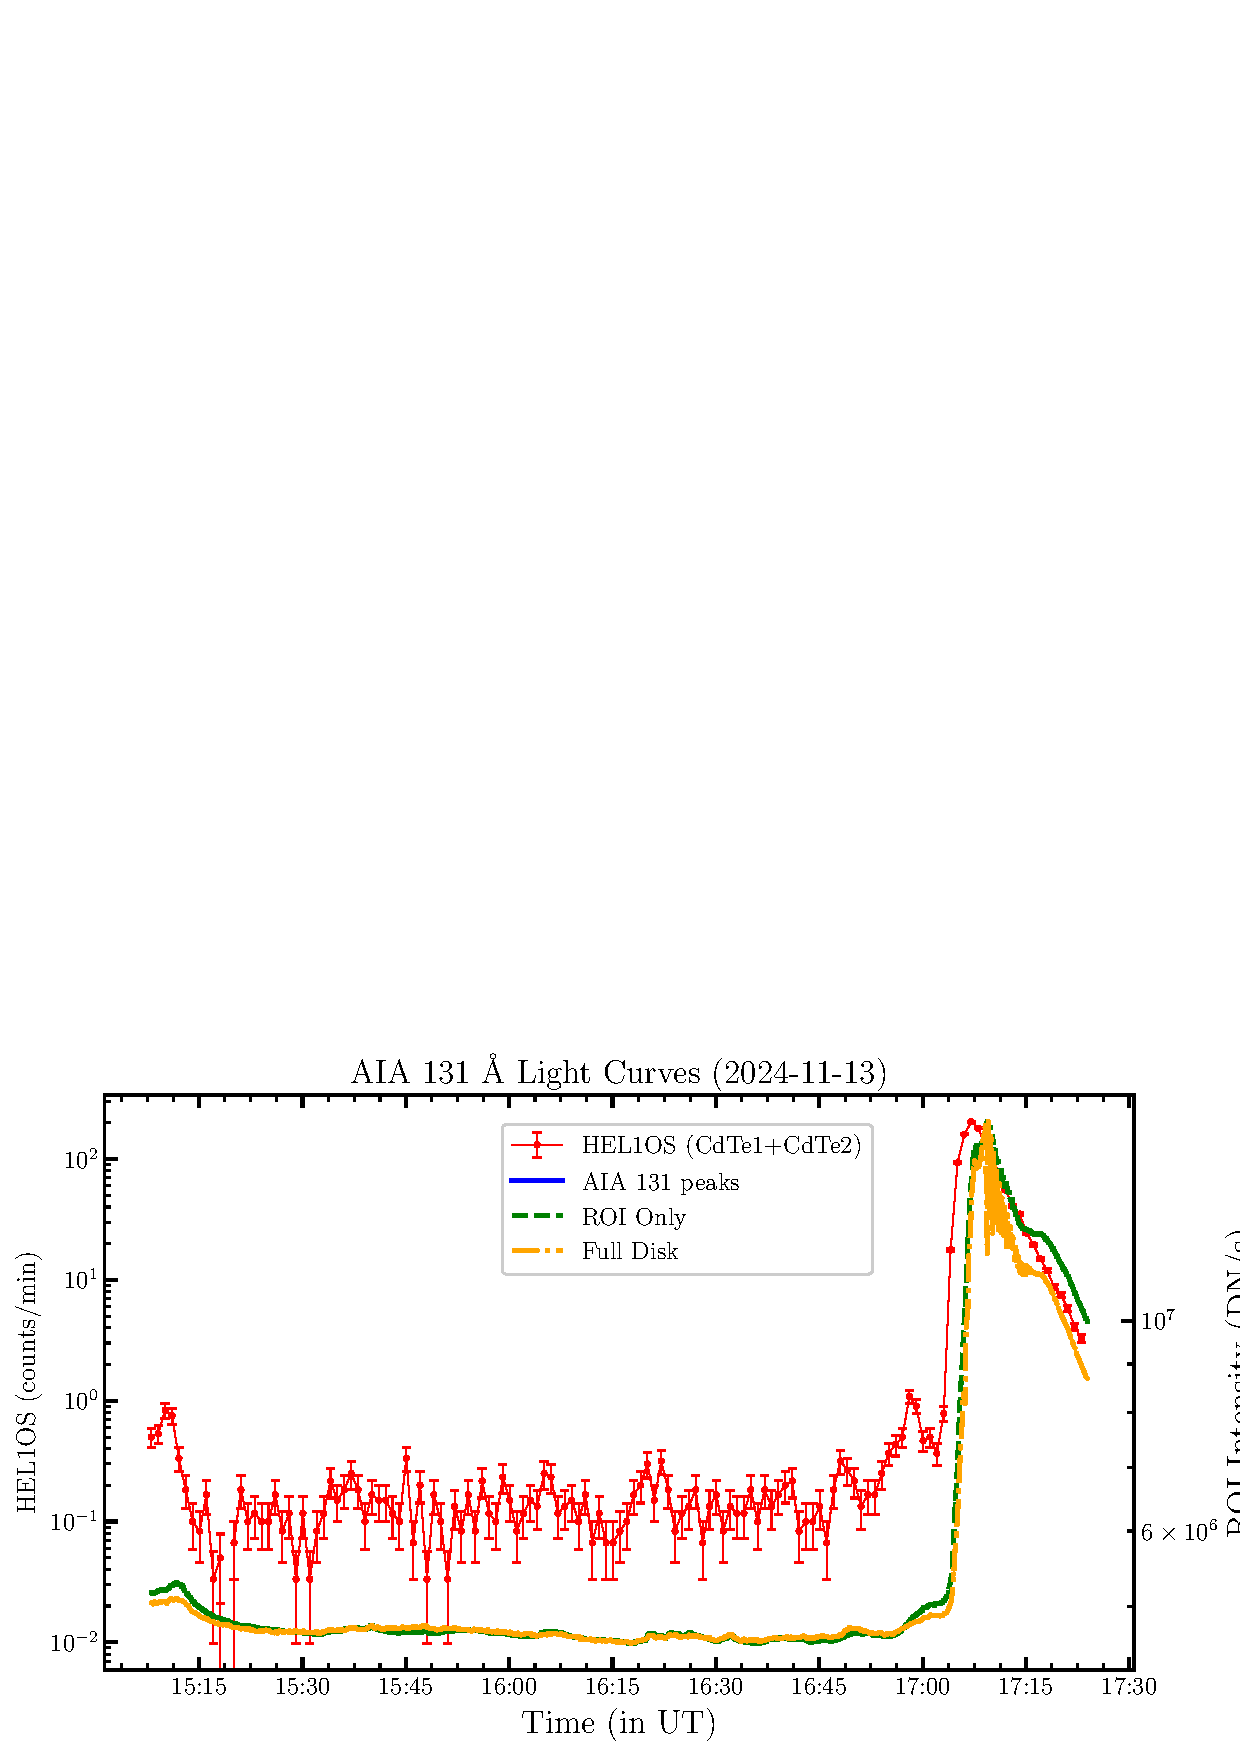
\includegraphics[width=1\linewidth]{Figures/c10_helios_aia_131_fd_roi_lc.pdf}
    \caption{Case 10: AIA 131 light curve}
    \label{fig:placeholder}
\end{figure}



\begin{figure}  
    \centering
    \includegraphics[width=1 \linewidth]{Figures/case1_lc.pdf}
    \caption{Case 1: June 1st flare}
    \label{fig:placeholder}
\end{figure}

\begin{figure}
    \centering
    \includegraphics[width=1\linewidth]{Figures/c1_aia_131_fd_roi_lc.png}
    \caption{AIA 131 light curve}
    \label{fig:placeholder}
\end{figure}

\begin{figure}
    \centering
    \includegraphics[width=1\linewidth]{Figures/case2_lc.png}
    \caption{Case 2 light curves}
    \label{fig:placeholder}
\end{figure}

\begin{figure}
    \centering
    \includegraphics[width=1\linewidth]{Figures/c2_aia_131_fd_roi_lc.png}
    \caption{AIA 131 light curve}
    \label{fig:placeholder}
\end{figure}


\begin{figure}
    \centering
    \includegraphics[width=1\linewidth]{Figures/case3_lc.png}
    \caption{Case 3 light curves}
    \label{fig:placeholder}
\end{figure}

\begin{figure}
    \centering
    \includegraphics[width=1\linewidth]{Figures/c3_aia_131_fd_roi_lc.png}
    \caption{AIA 131 light curve}
    \label{fig:placeholder}
\end{figure}

%%%%%%%%%%%%%%%%%%%%%%%%%%%%%%%%%%%%%%%%%%%%%%%%%%



% Don't change these lines
\bsp	% typesetting comment
\label{lastpage}

\end{document}

% End of mnras_template.tex
